\documentclass{article}
\usepackage[T1]{fontenc}
\usepackage{lmodern}
\usepackage[utf8]{inputenc}
\usepackage{caption}
\usepackage{geometry}
\geometry{left=2cm,right=2cm,top=2cm,bottom=3cm}

\usepackage[spanish,es-tabla]{babel}

\usepackage{url}
\usepackage{multirow}
\usepackage{siunitx}
\usepackage{amsmath}
\usepackage{float}
\usepackage{graphicx}
\usepackage{booktabs,array}
\newcolumntype{L}[1]{>{\raggedright\arraybackslash}p{#1}}
\usepackage[authoryear,round]{natbib}
\setcitestyle{aysep={,},notesep={: }}
\usepackage{fancyhdr}
\usepackage{hyperref}
\setlength{\parindent}{0pt}
\setlength{\parskip}{0.5em}
\usepackage{adjustbox}
\hypersetup{hidelinks,pdfauthor={Benjamín García, Luis Noriega y Matías Stierling},pdftitle={Planificación de la colocación de una fundación de hormigón masivo}}
\urlstyle{same}

% Tablas compactas: interlineado simple dentro de tablas
\usepackage{etoolbox}
\AtBeginEnvironment{tabular}{\linespread{1}\selectfont}
\captionsetup{font=small,labelfont=bf,skip=6pt}
% Separación compacta entre figuras/tablas y texto.
\setlength{\textfloatsep}{10pt plus 2pt minus 2pt}
\setlength{\intextsep}{10pt plus 2pt minus 2pt}
\renewcommand{\topfraction}{0.9}
\renewcommand{\bottomfraction}{0.8}
\renewcommand{\textfraction}{0.08}
\renewcommand{\floatpagefraction}{0.75}
\setlength{\floatsep}{8pt plus 2pt minus 2pt}

\def\unidad{Universidad de los Andes}
\def\programa{Facultad de Ingenier\'ia y Ciencias Aplicadas}
\def\titulo{Planificación de la colocación de una fundación de hormigón masivo}
\def\subtitulo{Métodos Computacionales en IOC}
\def\autores{
    Benjamín García \\
    Luis Noriega\\
    Matías Stierling\\
    [0.4cm]
    \normalsize Grupo $6$\\
}
\def\fecha{$23$ de noviembre de $2026$}
\def\lugar{
    Santiago,
    Chile
}

\pagestyle{fancy}
\fancyhf{}
\chead{Métodos Computacionales en IOC \vspace{0.3cm}}
\lhead{
\includegraphics[width=3cm]{Imagenes/marca_principal.jpg}}
\lfoot{\scriptsize Facultad de Ingenier\'ia y Ciencias Aplicadas\\Universidad de los Andes}
\rfoot{\thepage}
\renewcommand{\footrulewidth}{0.5pt}
\addtolength{\headheight}{1.5cm}
\renewcommand{\baselinestretch}{1.5}
% Reservar espacio para la línea y las dos líneas de texto del pie.
\addtolength{\textheight}{-24pt}
\setlength{\footskip}{38pt}

% Conservar juntos los renglones de cada párrafo al paginar.
\interlinepenalty=10000
\raggedbottom
\begin{document}

\hypersetup{pageanchor=false}
\begin{titlepage}
    \centering
    \linespread{1.12}\selectfont
    \setlength{\parskip}{0.15em}

    % --- Logo institucional ---
    \vspace*{1.0cm}
    
\includegraphics[width=0.32\linewidth]{Imagenes/marca_principal.jpg}\par
    \vspace{0.8cm}

    % --- Unidad y programa ---
    \rule{\linewidth}{0.4pt}\par
    \vspace{0.45cm}
    {\large\scshape\unidad\par}
    \vspace{0.20cm}
    {\large\scshape\programa\par}
    \vspace{0.45cm}
    \rule{\linewidth}{0.4pt}\par

    \vspace{1.0cm}

    % --- Título y subtítulo ---
    {\huge\bfseries\titulo\par}
    \vspace{0.8cm}
    {\Large\subtitulo\par}
    {\large Artículo académico final (F01)\par}

    \vfill

    % --- Autores ---
    {\large\autores\par}
    \vspace{1.0cm}

    % --- Lugar y fecha ---
    \rule{\linewidth}{0.4pt}\par
    \vspace{0.4cm}
    {\large\lugar\par}
    {\large\fecha\par}
    \vspace{0.6cm}

\end{titlepage}

\newpage
\pagenumbering{gobble} % Oculta el número de página de índice y resumen

\section*{Resumen}
La colocación continua de una fundación de hormigón masivo acorta la jornada de construcción, pero obliga a controlar el calor que se acumula en el interior y las diferencias de temperatura que aparecen al enfriarse sus superficies. Se estudió una fundación de aerogenerador de $636{,}775\,\mathrm{m^3}$ para el sitio docente de Los Ángeles, Chile. Un modelo de volúmenes finitos representó la geometría del proyecto, la colocación en once capas, las protecciones y nueve circuitos de refrigeración. Se combinaron ocho curvas de hidratación obtenidas de ensayos de probeta con tres historias meteorológicas del reanálisis ERA5. Entre los planes evaluados, la colocación continua a $60\,\mathrm{m^3/h}$ terminó en $10{,}61\,\mathrm h$, unos $58$ minutos antes que la alternativa de $55\,\mathrm{m^3/h}$. Con la última manta hasta los $21$ días de edad de cada capa y sombra posterior, ninguno de los $24$ escenarios superó los límites docentes de $70\,^\circ\mathrm C$ o $20\,\mathrm K$ durante los $28$ días de seguimiento. Con sombra y retiro a los $15$ días, cinco escenarios superaron al menos un límite en la malla de comparación. La recomendación depende de que en obra se alcancen la temperatura de colocación, la refrigeración y la protección solar previstas.

\textbf{Palabras clave}\quad hormigón masivo, calor de hidratación, control térmico, volúmenes finitos, planificación de la colocación

\clearpage
{\small\linespread{1.05}\selectfont\setlength{\parskip}{0pt}\tableofcontents\par}

\newpage
\pagenumbering{arabic} % Empieza a contar las páginas desde la introducción
\hypersetup{pageanchor=true}
\section{Introducción}
\label{sec:introduccion}

En una fundación de hormigón masivo, la hidratación del cemento libera calor en todo el volumen, mientras que su disipación ocurre principalmente por las superficies. El núcleo puede seguir caliente cuando la cara exterior ya se está enfriando. En fundaciones de aerogeneradores, \citet{ju2019} observaron esta diferencia y utilizaron mediciones a distintas profundidades para evaluar el control térmico.

El plazo de colocación y el control térmico están relacionados. Colocar más despacio modifica las edades relativas de las capas y la hora a la que quedan expuestas al ambiente. A su vez, retirar la aislación cuando el núcleo sigue caliente puede ampliar el diferencial \citep{ichControlTermico}. En una fundación de puente, \citet{sargam2019} contrastaron las temperaturas calculadas con mediciones de obra y mostraron la sensibilidad de la evolución térmica a los materiales y a las condiciones constructivas.

Este estudio examina si es posible sostener la mayor tasa de colocación disponible sin exceder el riesgo térmico admitido. La hipótesis de trabajo es que una colocación continua puede cumplir los criterios docentes si la refrigeración y la protección de las superficies se mantienen durante las etapas críticas. Para evaluarla se compara cada plan bajo las mismas combinaciones de hidratación y clima.

\subsection{Objetivo general}
Identificar el plan de colocación de menor duración entre las alternativas consideradas para la fundación del caso docente en Los Ángeles, región del Biobío, manteniendo una probabilidad conjunta no mayor que el $5~\%$ de exceder una temperatura de $70\,^{\circ}\mathrm{C}$ o un diferencial térmico de $20\,\mathrm{K}$, bajo el modelo de incertidumbre adoptado. Estos límites corresponden a criterios académicos.

\subsection{Objetivos específicos}
\begin{itemize}
    \item Documentar la procedencia de los datos y los
    supuestos del modelo térmico.
    \item Verificar el método mediante casos conocidos,
    balances energéticos y análisis de sensibilidad
    espacial y temporal.
    \item Comparar la duración de colocación y las
    probabilidades de excedencia de los planes bajo
    escenarios comunes.
    \item Formular un plan de control térmico con
    monitoreo y acciones de contingencia.
\end{itemize}
\clearpage
\section{Caso de estudio y datos}
\label{sec:caso-datos}

%-------------------------------------------
\subsection{Emplazamiento y geometría de la fundación}
\label{sec:emplazamiento-geometria}
%-------------------------------------------

El caso de estudio corresponde a una fundación de hormigón masivo para un aerogenerador, evaluada bajo las condiciones meteorológicas del sector de Los Ángeles, región del Biobío. El sitio de referencia es el Parque Eólico El Rosal y el punto de consulta climática se fija en la latitud $-37{,}277929^{\circ}$ y la longitud $-72{,}368271^{\circ}$. Estas coordenadas representan el punto meteorológico del caso docente y no la ubicación exacta de una fundación construida. De esta manera, el estudio combina una geometría común del proyecto académico con condiciones ambientales asociadas al sitio asignado.

La geometría se obtiene del archivo oficial de trabajo \texttt{fundacion.ifc}, conservado en el repositorio. El modelo contiene cinco objetos de clase \texttt{IfcFooting}, denominados \texttt{Vertida\_01} a \texttt{Vertida\_05}, que conforman un cuerpo de base octogonal, una transición de sección decreciente y un pedestal superior cilíndrico, como se muestra en la Figura~\ref{fig:geometria-ifc}. La extensión máxima en planta es de $18\times18\,\mathrm{m}$ y la altura total alcanza $4{,}30\,\mathrm{m}$. El pedestal ocupa el tramo entre las cotas $3{,}30$ y $4{,}30\,\mathrm{m}$, con un diámetro nominal de $7\,\mathrm{m}$.

\begin{figure}[htbp]
  \centering
  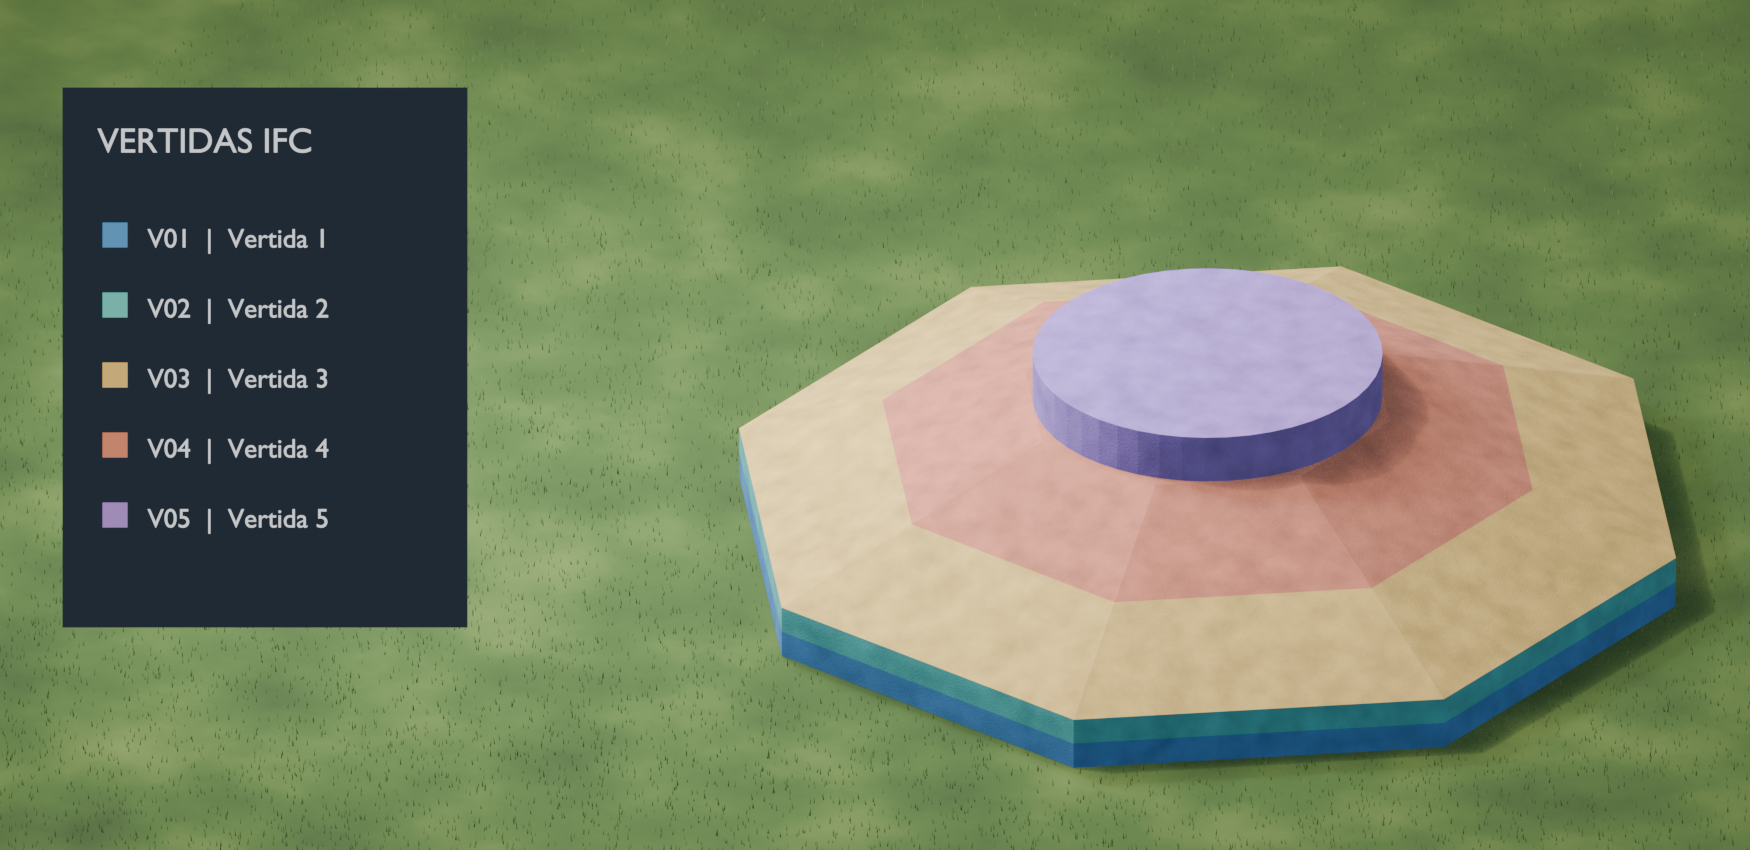
\includegraphics[width=0.85\linewidth]{Imagenes/geometria_ifc.png}
  \caption{Geometría de la fundación y vertidas definidas en el modelo IFC}
  \label{fig:geometria-ifc}
  \captionsetup{skip=2pt}
  \caption*{Fuente: elaboración propia en Blender/Bonsai a partir de \texttt{fundacion.ifc}.}
\end{figure}

La Tabla~\ref{tab:geometria-ifc} resume las cotas, las dimensiones envolventes y los volúmenes obtenidos de las superficies trianguladas del IFC. La suma de los volúmenes de las cinco vertidas es de $636{,}775\,\mathrm{m^3}$. Las dimensiones envolventes indican la extensión máxima de cada pieza; su producto no representa el volumen del sólido, debido a la forma octogonal y a las superficies inclinadas. Esta distinción evita sustituir la geometría real del modelo por bloques rectangulares de mayor volumen.

\begin{table}[htbp]
  \centering
  \caption{Características geométricas de los objetos de la fundación}
  \label{tab:geometria-ifc}
  \small
  \begin{tabular}{lccc}
    \toprule
    Objeto & Intervalo de cota [m] & Envolvente $x\times y\times z$ [m] & Volumen [$\mathrm{m^3}$] \\
    \midrule
    \texttt{Vertida\_01} & $0{,}00$--$0{,}55$ & $18{,}00\times18{,}00\times0{,}55$ & $147{,}626$ \\
    \texttt{Vertida\_02} & $0{,}55$--$1{,}10$ & $18{,}00\times18{,}00\times0{,}55$ & $147{,}626$ \\
    \texttt{Vertida\_03} & $1{,}10$--$2{,}20$ & $18{,}00\times18{,}00\times1{,}10$ & $214{,}224$ \\
    \texttt{Vertida\_04} & $2{,}20$--$3{,}30$ & $12{,}50\times12{,}50\times1{,}10$ & $88{,}925$ \\
    \texttt{Vertida\_05} & $3{,}30$--$4{,}30$ & $7{,}00\times7{,}00\times1{,}00$ & $38{,}375$ \\
    \midrule
    Conjunto & $0{,}00$--$4{,}30$ & $18{,}00\times18{,}00\times4{,}30$ & $636{,}775$ \\
    \bottomrule
  \end{tabular}
  \captionsetup{skip=2pt}
  \caption*{Fuente: extracción propia del archivo IFC.}
\end{table}

Se distinguen la base en contacto con el terreno, las superficies laterales y la coronación expuestas al ambiente. La representación térmica considera el volumen de hormigón, sin resolver explícitamente las armaduras ni los anclajes del aerogenerador.

La partición geométrica del IFC se mantiene como referencia de identidad y forma, pero se distingue de la secuencia constructiva evaluada. Aunque los objetos conservan el nombre de vertidas, la propuesta distribuye la colocación en once capas físicas sin alterar la geometría final. La definición de esas capas, su cronología y los controles térmicos se presentan en los apartados siguientes. Asimismo, la comparación entre el volumen geométrico y el volumen representado por la malla se desarrolla al describir la voxelización.


%-------------------------------------------
%-------------------------------------------
\subsection{Representación BIM y voxelización}
\label{sec:BIM-Voxelización}
%-------------------------------------------

El flujo de trabajo parte del modelo BIM almacenado en formato IFC y transforma su geometría en una malla cartesiana para el cálculo térmico. La lectura se realiza con IfcOpenShell, que permite obtener los vértices y las caras trianguladas de los sólidos \citep{ifcopenshellGeometria}. Se aplican las posiciones de los objetos y la conversión de unidades a metros, conservando las coordenadas locales del proyecto. Los nombres y los identificadores de los objetos se mantienen para vincular la representación numérica con el archivo de origen.

La información geométrica utilizada comprende las superficies trianguladas, las dimensiones y la posición relativa de las cinco piezas. El lector también recupera sus propiedades constructivas, pero el cálculo del plan adoptado utiliza un cronograma externo de once capas, junto con las temperaturas de colocación y los controles definidos para la comparación. Por tanto, los valores iniciales almacenados en los campos del IFC no se adoptan automáticamente como condiciones del estudio. Las propiedades térmicas del material y los datos ambientales se incorporan desde archivos de configuración independientes.

La voxelización consiste en dividir la caja envolvente del conjunto en celdas cúbicas de lado $h$. El origen de la malla coincide con el mínimo geométrico del IFC, aproximadamente $(-9,-9,0)\,\mathrm{m}$, y se mantiene al refinar. Cada centro de celda se clasifica respecto de las superficies trianguladas: la celda se considera ocupada si el centro está dentro de alguno de los sólidos o sobre su frontera, con una tolerancia geométrica de $10^{-7}\,\mathrm{m}$. La pertenencia a varios objetos no duplica su ocupación. 

Este criterio asigna el volumen completo de la celda y no calcula fracciones de intersección, por lo que aproxima las superficies curvas e inclinadas mediante un contorno escalonado. Para cuantificar esta aproximación se calcula el volumen discretizado como:
\begin{equation}
    V_h=N_h \cdot h^3
\end{equation}
tal que $N_h$ es el número de celdas ocupadas y $h$ es el lado de cada celda. Este volumen se compara con la referencia geométrica $V_{\mathrm{IFC}}=636{,}775\,\mathrm{m^3}$, obtenida como la suma de los volúmenes de las piezas trianguladas.
La diferencia firmada es: 
\begin{equation}
    \Delta V=V_h-V_{\mathrm{IFC}}
\end{equation}
y su magnitud relativa es:
\begin{equation}
    \varepsilon_V=\frac{|\Delta V|}{V_{\mathrm{IFC}}} \cdot 100
\end{equation}
tal que $\varepsilon_V$ es la magnitud de la diferencia relativa expresada en porcentaje. La Tabla~\ref{tab:volumen-voxelizacion} presenta los valores recuperados de las geometrías guardadas para las dos resoluciones utilizadas. Las diferencias se calculan con los valores sin redondear; el redondeo se aplica únicamente para su presentación.

\begin{table}[htbp]
  \centering
  \caption{Comparación del volumen geométrico y discretizado de la fundación}
  \label{tab:volumen-voxelizacion}
  \small
  \begin{tabular}{ccccc}
    \toprule
    $h$ [m] & $N_h$ & $V_h$ [$\mathrm{m^3}$] & $\Delta V$ [$\mathrm{m^3}$] & $\varepsilon_V$ [\%] \\
    \midrule
    $0{,}40$ & $10\,011$ & $640{,}704$ & $+3{,}929$ & $0{,}617$ \\
    $0{,}20$ & $79\,868$ & $638{,}944$ & $+2{,}169$ & $0{,}341$ \\
    \bottomrule
  \end{tabular}
  \captionsetup{skip=2pt}
  \caption*{Fuente: elaboración propia a partir de las geometrías archivadas.}
\end{table}

En ambas mallas el volumen discretizado supera al geométrico, aunque la diferencia disminuye al pasar de $0{,}40$ a $0{,}20\,\mathrm{m}$. Este resultado caracteriza la aproximación global del volumen, pero no demuestra por sí solo la exactitud de las superficies ni la convergencia de las temperaturas. Para calcular la duración de colocación se conserva el volumen físico del plan, sin sustituirlo por el volumen voxelizado; así, un cambio de malla no modifica artificialmente el objetivo constructivo.

Finalmente, las celdas ocupadas se agrupan por altura en las once capas del plan, manteniendo esa misma partición física en ambas resoluciones. La máscara geométrica representa la fundación completa y se distingue del dominio activo: durante el cálculo solo participan las capas cuya colocación ya se ha activado. La activación y la identificación de las caras exteriores permiten actualizar las superficies de intercambio a medida que avanza la construcción. Su formulación térmica se desarrolla en las secciones de modelo continuo y discretización.

%-------------------------------------------
%-------------------------------------------
\subsection{Parámetros térmicos y condiciones de colocación}
\label{sec:Parametros y condiciones}
%-------------------------------------------

Para comparar los planes en las mismas condiciones, se conservan los datos del material, del ambiente y de los sistemas de protección y refrigeración; entre las dos alternativas cambia la tasa de colocación. Las Tablas~\ref{tab:param-materiales} a~\ref{tab:param-plan} reúnen estos parámetros y señalan su procedencia. La clasificación bibliográfico corresponde a valores publicados; ajustado, a resultados obtenidos al ajustar un modelo a datos; y supuesto, a valores o decisiones adoptados para el estudio. Un dato se presenta como medido únicamente si se dispone de antecedentes que acrediten su medición.

La densidad y el calor específico se toman del archivo docente de hidratación \citep{fuentesDocentes}. La conductividad del hormigón, en cambio, se adopta como un valor fijo que no se ajustó a mediciones de la fundación. Ese archivo también entrega las curvas que describen cuánto calor genera el hormigón a medida que envejece; su origen y tratamiento se explican en el apartado siguiente.

Para la madera y las mantas se utilizan los valores publicados para AraucoPly y Aislanglass \citep{araucoCatalogo,volcanCES}. La referencia de AraucoPly corresponde al catálogo internacional de esa familia de tableros, por lo que su aplicación al producto utilizado en obra requiere comprobar que sus características sean equivalentes. En ambos materiales, la información publicada permite representar su resistencia térmica, pero no sustituye la comprobación del montaje de las protecciones.

\begin{table}[htbp]
  \centering
  \caption{Propiedades del hormigón y de las protecciones térmicas}
  \label{tab:param-materiales}
  \small
  \setlength{\tabcolsep}{4pt}
  \begin{tabular}{p{1.4cm}p{4.0cm}p{2.1cm}p{2.0cm}p{3.8cm}p{2.7cm}}
    \toprule
    Símbolo & Significado & Unidad & Valor & Procedencia & Clasificación \\
    \midrule
    $\rho$ & Densidad del hormigón & $\mathrm{kg\,m^{-3}}$ & $2\,476$ & Archivo docente & Supuesto adoptado \\
    $c_p$ & Calor específico & $\mathrm{J\,kg^{-1}\,K^{-1}}$ & $1\,023$ & Archivo docente & Supuesto adoptado \\
    $k_c$ & Conductividad del hormigón & $\mathrm{W\,m^{-1}\,K^{-1}}$ & $2$ & Configuración térmica & Supuesto \\
    $\dot q_{h,m}(a)$ & Fuente por edad y curva & $\mathrm{W\,m^{-3}}$ & $8$ funciones tabuladas & Archivo docente & Ajustado \\
    $e_m$ & Espesor de madera & $\mathrm{m}$ & $0{,}018$ & Referencia AraucoPly & Bibliográfico \\
    $k_m$ & Conductividad de madera & $\mathrm{W\,m^{-1}\,K^{-1}}$ & $0{,}158$ & AraucoPly, tabla $11$ & Bibliográfico \\
    $e_a$ & Espesor de cada manta & $\mathrm{m}$ & $0{,}040$ & Ficha Aislanglass & Bibliográfico \\
    $k_a$ & Conductividad de cada manta & $\mathrm{W\,m^{-1}\,K^{-1}}$ & $0{,}042$ & Ficha Aislanglass & Bibliográfico \\
    \bottomrule
  \end{tabular}
  \captionsetup{skip=2pt}
  \caption*{Fuente: Archivo docente de hidratación, documentación de ARAUCO y Volcán, y configuración del estudio.}
\end{table}

Para representar la pérdida de calor hacia el suelo, se supone que el terreno mantiene una temperatura constante y que el calor atraviesa una distancia equivalente de suelo. No se calcula cómo se calienta o enfría el terreno con el tiempo. El intercambio con el aire depende del viento y se estima con la relación de McAdams presentada en la documentación de EnergyPlus \citep{energyplusMcAdams}, expresada en unidades SI como:
\begin{equation}
    h_c(t)=5{,}7+3{,}8~v_2(t)
\end{equation}
tal que $v_2(t)$ es la velocidad horaria del viento en $\mathrm{m\,s^{-1}}$, referida a una altura de $2\,\mathrm{m}$, y $h_c(t)$ relaciona el intercambio de calor con la diferencia de temperatura entre la superficie y el aire. 
\newpage
La altura de referencia y el exponente usado para ajustar el viento se adoptan como supuestos. También se fijan la fracción de radiación solar absorbida por la superficie, denominada absortancia; su capacidad de emitir radiación térmica, representada por la emisividad; y la fracción de radiación solar reflejada por el entorno, o albedo. Estos valores no proceden de mediciones del acabado de la fundación. La Tabla~\ref{tab:param-ambiente} los reúne junto con los parámetros del suelo y de la sombra. El subíndice de $h_c$ permite distinguir este coeficiente del lado de celda $h$.

\begin{table}[htbp]
  \centering
  \caption{Parámetros del suelo y del intercambio con el ambiente}
  \label{tab:param-ambiente}
  \small
  \setlength{\tabcolsep}{4pt}
  \begin{tabular}{p{1.4cm}p{3.5cm}p{2.1cm}p{1.8cm}p{3.8cm}p{2.2cm}}
    \toprule
    Símbolo & Significado & Unidad & Valor & Procedencia & Clasificación \\
    \midrule
    $T_g$ & Temperatura del reservorio de suelo & $^{\circ}\mathrm{C}$ & $15$ & Configuración del suelo & Supuesto \\
    $L_g$ & Longitud equivalente de suelo & $\mathrm{m}$ & $0{,}50$ & Configuración del suelo & Supuesto \\
    $k_g$ & Conductividad equivalente del suelo & $\mathrm{W\,m^{-1}\,K^{-1}}$ & $1{,}2$ & Configuración del suelo & Supuesto \\
    $h_c(t)$ & Coeficiente convectivo & $\mathrm{W\,m^{-2}\,K^{-1}}$ & Variable & McAdams, según EnergyPlus & Bibliográfico \\
    $z_v$ & Altura representativa del viento & $\mathrm{m}$ & $2$ & Configuración ambiental & Supuesto \\
    $\gamma_v$ & Exponente del perfil de viento & Adimensional & $0{,}14$ & Configuración ambiental & Supuesto \\
    $\alpha_{\mathrm{SW}}$ & Absortancia solar exterior & Adimensional & $0{,}60$ & Configuración radiativa & Supuesto \\
    $\varepsilon$ & Emisividad de onda larga & Adimensional & $0{,}90$ & Configuración radiativa & Supuesto \\
    $r_g$ & Albedo del entorno & Adimensional & $0{,}20$ & Configuración radiativa & Supuesto \\
    $\tau_{\mathrm{SW}}$ & Transmitancia solar de la sombra & Adimensional & $0{,}10$ & Protección idealizada & Supuesto \\
    \bottomrule
  \end{tabular}
  \captionsetup{skip=2pt}
  \caption*{Fuente: Documentación de EnergyPlus y configuración del estudio.}
\end{table}
Los planes parten del $19$ de noviembre de $2026$ a las $10{:}00$, con desfase UTC$-03{:}00$. La propuesta considera dos frentes de hasta $30\,\mathrm{m^3/h}$ cada uno, sin esperas entre las once capas y con hormigón colocado a $12\,^{\circ}\mathrm{C}$. Los laterales se cubren con madera y dos mantas, mientras que la cara superior recibe las dos mantas sin madera. El retiro se cuenta desde la colocación de cada capa: la madera permanece $72\,\mathrm{h}$, la primera manta $240\,\mathrm{h}$ y la segunda $504\,\mathrm{h}$. Al retirar la última manta se incorpora una sombra idealizada que deja pasar el $10~\%$ de la radiación solar y se conserva hasta el final del seguimiento de $672\,\mathrm{h}$, manteniendo las demás condiciones de intercambio. Las edades de retiro forman parte de la programación simulada. Los resultados respaldan el cumplimiento de los criterios térmicos al mantener la última manta hasta las $504\,\mathrm{h}$ de edad de cada capa y aplicar posteriormente la sombra, bajo los escenarios y supuestos evaluados. No se buscó determinar la menor edad de retiro admisible. Su aplicación en obra requiere comprobar las temperaturas y la resistencia del hormigón.
\newpage

El efecto de los circuitos se incorpora como una extracción de calor distribuida en la zona refrigerable, con agua a temperatura uniforme y una potencia total limitada. Un circuito solo puede abrirse después de quedar cubierto por hormigón y cuando todos sus puntos de control alcanzan al menos $19\,^{\circ}\mathrm{C}$; se cierra si alguno baja a $18\,^{\circ}\mathrm{C}$ o menos. La diferencia entre ambas temperaturas evita aperturas y cierres repetidos alrededor de un único umbral. Este control puede actuar durante todo el seguimiento, sin una fecha fija de apagado general. El coeficiente $U_v$ representa el intercambio térmico equivalente adoptado: no se obtiene del caudal nominal de los ramales. El modelo no calcula el paso de calor a través de la pared del tubo y su contacto con el hormigón, ni el calentamiento del agua a lo largo del recorrido. Por ello, el comportamiento calculado todavía requiere una comprobación del diseño hidráulico y de la transferencia real de calor.

\begin{table}[htbp]
  \centering
  \caption{Condiciones de colocación y refrigeración adoptadas}
  \label{tab:param-plan}
  \small
  \setlength{\tabcolsep}{4pt}
  \begin{tabular}{p{1.4cm}p{3.8cm}p{2.1cm}p{2.0cm}p{3.7cm}p{2.8cm}}
    \toprule
    Símbolo & Significado & Unidad & Valor o conjunto & Procedencia & Clasificación \\
    \midrule
    $q$ & Tasa de colocación comparada & $\mathrm{m^3\,h^{-1}}$ & $55$ y $60$ & Familia de planes & Supuesto de capacidad \\
    $T_{\mathrm{col}}$ & Temperatura de colocación & $^{\circ}\mathrm{C}$ & $12$ & Configuración del plan & Supuesto \\
    $n_L$ & Número de capas físicas & Adimensional & $11$ & Partición adoptada & Supuesto de diseño \\
    $e_L$ & Espesor nominal de capa; última capa & $\mathrm{m}$ & $0{,}40$; $0{,}30$ & Partición adoptada & Supuesto de diseño \\
    $a_r$ & Edades de retiro: madera y mantas & $\mathrm{h}$ & $72$; $240$; $504$ & Protección evaluada & Supuesto de diseño \\
    $n_r$ & Número de circuitos & Adimensional & $9$ & Anteproyecto del equipo & Supuesto de diseño \\
    $T_w$ & Temperatura uniforme del agua & $^{\circ}\mathrm{C}$ & $18$ & Refrigeración equivalente & Supuesto \\
    $U_v$ & Coeficiente volumétrico de extracción & $\mathrm{W\,m^{-3}\,K^{-1}}$ & $5$ & Refrigeración equivalente & Supuesto \\
    $P_{\max}$ & Potencia máxima global & $\mathrm{kW}$ & $15$ & Refrigeración equivalente & Supuesto \\
    $V_r$ & Volumen refrigerable & $\mathrm{m^3}$ & $414{,}016$ & Máscara del anteproyecto & Supuesto de diseño \\
    $Q_r$ & Caudal nominal por ramal abierto & $\mathrm{L\,min^{-1}}$ & $18$ & Anteproyecto del equipo & Supuesto de diseño \\
    $Q_{\mathrm{tot}}$ & Caudal total con bypass & $\mathrm{L\,min^{-1}}$ & $162$ & Anteproyecto del equipo & Supuesto de diseño \\
    $T_{\mathrm{on}}$, $T_{\mathrm{off}}$ & Umbrales de apertura y cierre & $^{\circ}\mathrm{C}$ & $19$; $18$ & Control por histéresis & Supuesto de diseño \\
    \bottomrule
  \end{tabular}
  \captionsetup{skip=2pt}
  \caption*{Fuente: Configuración final del estudio y anteproyecto de circuitos del equipo.}
\end{table}


%-------------------------------------------
\subsection{Datos de hidratación y tratamiento de las ocho curvas}
\label{sec:Hidratación y curvas}
%-------------------------------------------

Para describir el calor de hidratación se utilizan las ocho curvas del archivo docente \texttt{source\_terms.txt}: \texttt{M1\_SS} a \texttt{M4\_SS} y \texttt{M1\_22A} a \texttt{M4\_22A}. Cada curva indica la potencia térmica generada por unidad de volumen de hormigón, en $\mathrm{W\,m^{-3}}$. Estos valores se estimaron a partir de registros de temperatura de probetas, ajustando un modelo para determinar la generación de calor que explica las temperaturas observadas \citep{fuentesDocentes}. Este procedimiento se denomina inversión. Las curvas entregadas ya son fuentes de calor, por lo que se incorporan sin volver a derivar una temperatura adiabática.
\newpage

El archivo describe probetas cilíndricas de radio $0{,}0375\,\mathrm{m}$ y altura $0{,}15\,\mathrm{m}$. Para estimar el calor generado se utilizó un modelo de volúmenes finitos que aprovecha la simetría del cilindro y considera sus pérdidas hacia el ambiente mediante una conductancia de borde fija de $2{,}5\,\mathrm{W\,m^{-2}\,K^{-1}}$. La curva se representó con B-splines cúbicos, es decir, funciones polinómicas unidas de forma suave, con $16$ funciones base. El ajuste incorporó regularización de Tikhonov, con una penalización de segundas diferencias de $0{,}05$, y correcciones de los desplazamientos de lectura de cada sensor. Estos procedimientos buscan controlar las oscilaciones del ajuste y las diferencias sistemáticas entre sensores. Se conservó ese procesamiento docente, sin repetirlo para el estudio de la fundación.

Las etiquetas \texttt{M1} a \texttt{M4} identifican las probetas. Las curvas \texttt{SS} corresponden a registros del $13$ al $20$ de abril de $2025$, y las \texttt{22A}, al $22$ de abril del mismo año. En ambos grupos se toma como edad cero el comienzo de la parte del registro que se conservó, situada dos horas después del inicio original. Ese instante se usa como aproximación del inicio de hidratación de cada capa. El calor de las dos horas descartadas no se reconstruye, lo que limita la representación de las primeras edades.

No se dispone de antecedentes suficientes para confirmar que las ocho curvas provengan de ensayos independientes de una misma dosificación. Se conservan como ocho respuestas posibles del material dentro del modelo, sin atribuirles una representatividad estadística que los datos no demuestran. Además, el archivo señala que las curvas \texttt{22A} tienen menor confianza, porque el sensor ambiental no explica adecuadamente la respuesta de las probetas a los cambios diarios de temperatura. El error de ajuste reportado, medido como raíz del error cuadrático medio, es de aproximadamente $0{,}4\,\mathrm{K}$ para \texttt{22A} y de $0{,}1$--$0{,}2\,\mathrm{K}$ para \texttt{SS}. Se mantienen las ocho curvas en la comparación, reconociendo que la calidad del ajuste difiere entre ambas campañas.

Se conserva cada serie hasta su última muestra disponible. Los valores \texttt{NaN} que aparecen después indican que el registro terminó; no se interpretan como mediciones de calor nulo. No se encontraron datos faltantes dentro de los tramos conservados ni se aplicó un nuevo suavizado. Las muestras están separadas por $600\,\mathrm{s}$, equivalentes a diez minutos, y se utiliza ese intervalo para evitar diferencias debidas al redondeo de las horas en el archivo. El calor acumulado se obtiene sumando el aporte entre muestras mediante la regla del trapecio:
\begin{equation}
    H_{m,j}=\sum_{r=0}^{j-1}
    \frac{\dot q_{m,r}+\dot q_{m,r+1}}{2}
    (a_{r+1}-a_r), \qquad H_{m,0}=0,
\end{equation}
tal que $m$ identifica la curva, $j$ y $r$ indican las posiciones de las muestras y $a_r$ es la edad en segundos. El valor $H_{m,j}$ representa el calor generado hasta esa edad por unidad de volumen de hormigón, en $\mathrm{J\,m^{-3}}$.

Para incorporar estos datos al cálculo, se unen con segmentos rectos los valores del calor acumulado $H_m(a)$. Así se puede obtener la energía generada entre dos edades, aunque no coincidan con las muestras originales. La pendiente de cada segmento representa la fuente efectiva utilizada en ese intervalo:
\begin{equation}
    \dot q_{h,m}(a)=\frac{H_{m,j+1}-H_{m,j}}{a_{j+1}-a_j},
    \qquad a_j\leq a<a_{j+1}.
\end{equation}
\newpage

Durante un paso que va de la edad $a_i$ a la edad $a_f$, el calor incorporado por unidad de volumen es:
\begin{equation}
    H_m(a_f)-H_m(a_i)
\end{equation}
De esta forma, el aporte depende del calor acumulado entre ambos instantes y se conserva aunque el paso de cálculo difiera del intervalo de los datos. La Figura~\ref{fig:hidratacion-fuentes} muestra las ocho curvas entregadas, las fuentes utilizadas durante las primeras $48\,\mathrm{h}$ y sus calores acumulados.

La Tabla~\ref{tab:hidratacion-calor} resume el máximo de cada curva y su calor total. Al integrar las fuentes se recuperan, a la precisión de los archivos, los acumulados guardados en los ocho CSV. El mismo resultado se obtiene al sumar los aportes con intervalos de $300\,\mathrm{s}$. Esta comprobación confirma que el tratamiento conserva la energía de los datos; no permite concluir que el ajuste de las probetas o las temperaturas de la fundación hayan sido validados con mediciones independientes.

Después de la última muestra se mantiene constante el calor acumulado. Esto equivale a suponer que no se genera más calor después de aproximadamente $240{,}333\,\mathrm{h}$ para \texttt{SS} y $163\,\mathrm{h}$ para \texttt{22A}. Se trata de una hipótesis para completar el período sin datos, y no de una observación del fin de la hidratación. De hecho, la última muestra de \texttt{M1\_SS} todavía indica una fuente de $1{,}57\,\mathrm{W\,m^{-3}}$.

En cada simulación se asigna una misma curva completa a todas las capas, pero la edad comienza a contarse al activar cada una. Esto supone que el material de toda la fundación comparte una misma respuesta de hidratación. La generación de calor depende únicamente de esa edad, sin modificar su velocidad según la temperatura calculada. Cada curva se conserva por separado: no se combinan partes de distintas series ni se utiliza una curva promedio para reemplazarlas. Los pesos asignados y sus consecuencias se explican en la sección de incertidumbre.

\begin{table}[htbp]
  \centering
  \caption{Duración de registro, máximos tabulados y calor acumulado de las fuentes de hidratación}
  \label{tab:hidratacion-calor}
  \small
  \begin{tabular}{lccc}
    \toprule
    Curva & Edad final [h] & Máximo tabulado [$\mathrm{W\,m^{-3}}$] & Calor [$\mathrm{MJ\,m^{-3}}$] \\
    \midrule
    \texttt{M1\_SS}  & $240{,}333$ & $467{,}75$ & $88{,}148$ \\
    \texttt{M2\_SS}  & $240{,}333$ & $531{,}11$ & $95{,}715$ \\
    \texttt{M3\_SS}  & $240{,}333$ & $553{,}01$ & $94{,}149$ \\
    \texttt{M4\_SS}  & $240{,}333$ & $568{,}94$ & $100{,}166$ \\
    \texttt{M1\_22A} & $163{,}000$ & $473{,}38$ & $61{,}212$ \\
    \texttt{M2\_22A} & $163{,}000$ & $625{,}29$ & $82{,}446$ \\
    \texttt{M3\_22A} & $163{,}000$ & $589{,}70$ & $73{,}289$ \\
    \texttt{M4\_22A} & $163{,}000$ & $596{,}08$ & $73{,}628$ \\
    \bottomrule
  \end{tabular}
  \captionsetup{skip=2pt}
  \caption*{Fuente: Elaboración propia a partir del archivo docente y de los acumulados conservados en el repositorio.}
\end{table}
\newpage

\begin{figure}[htbp]
  \centering
  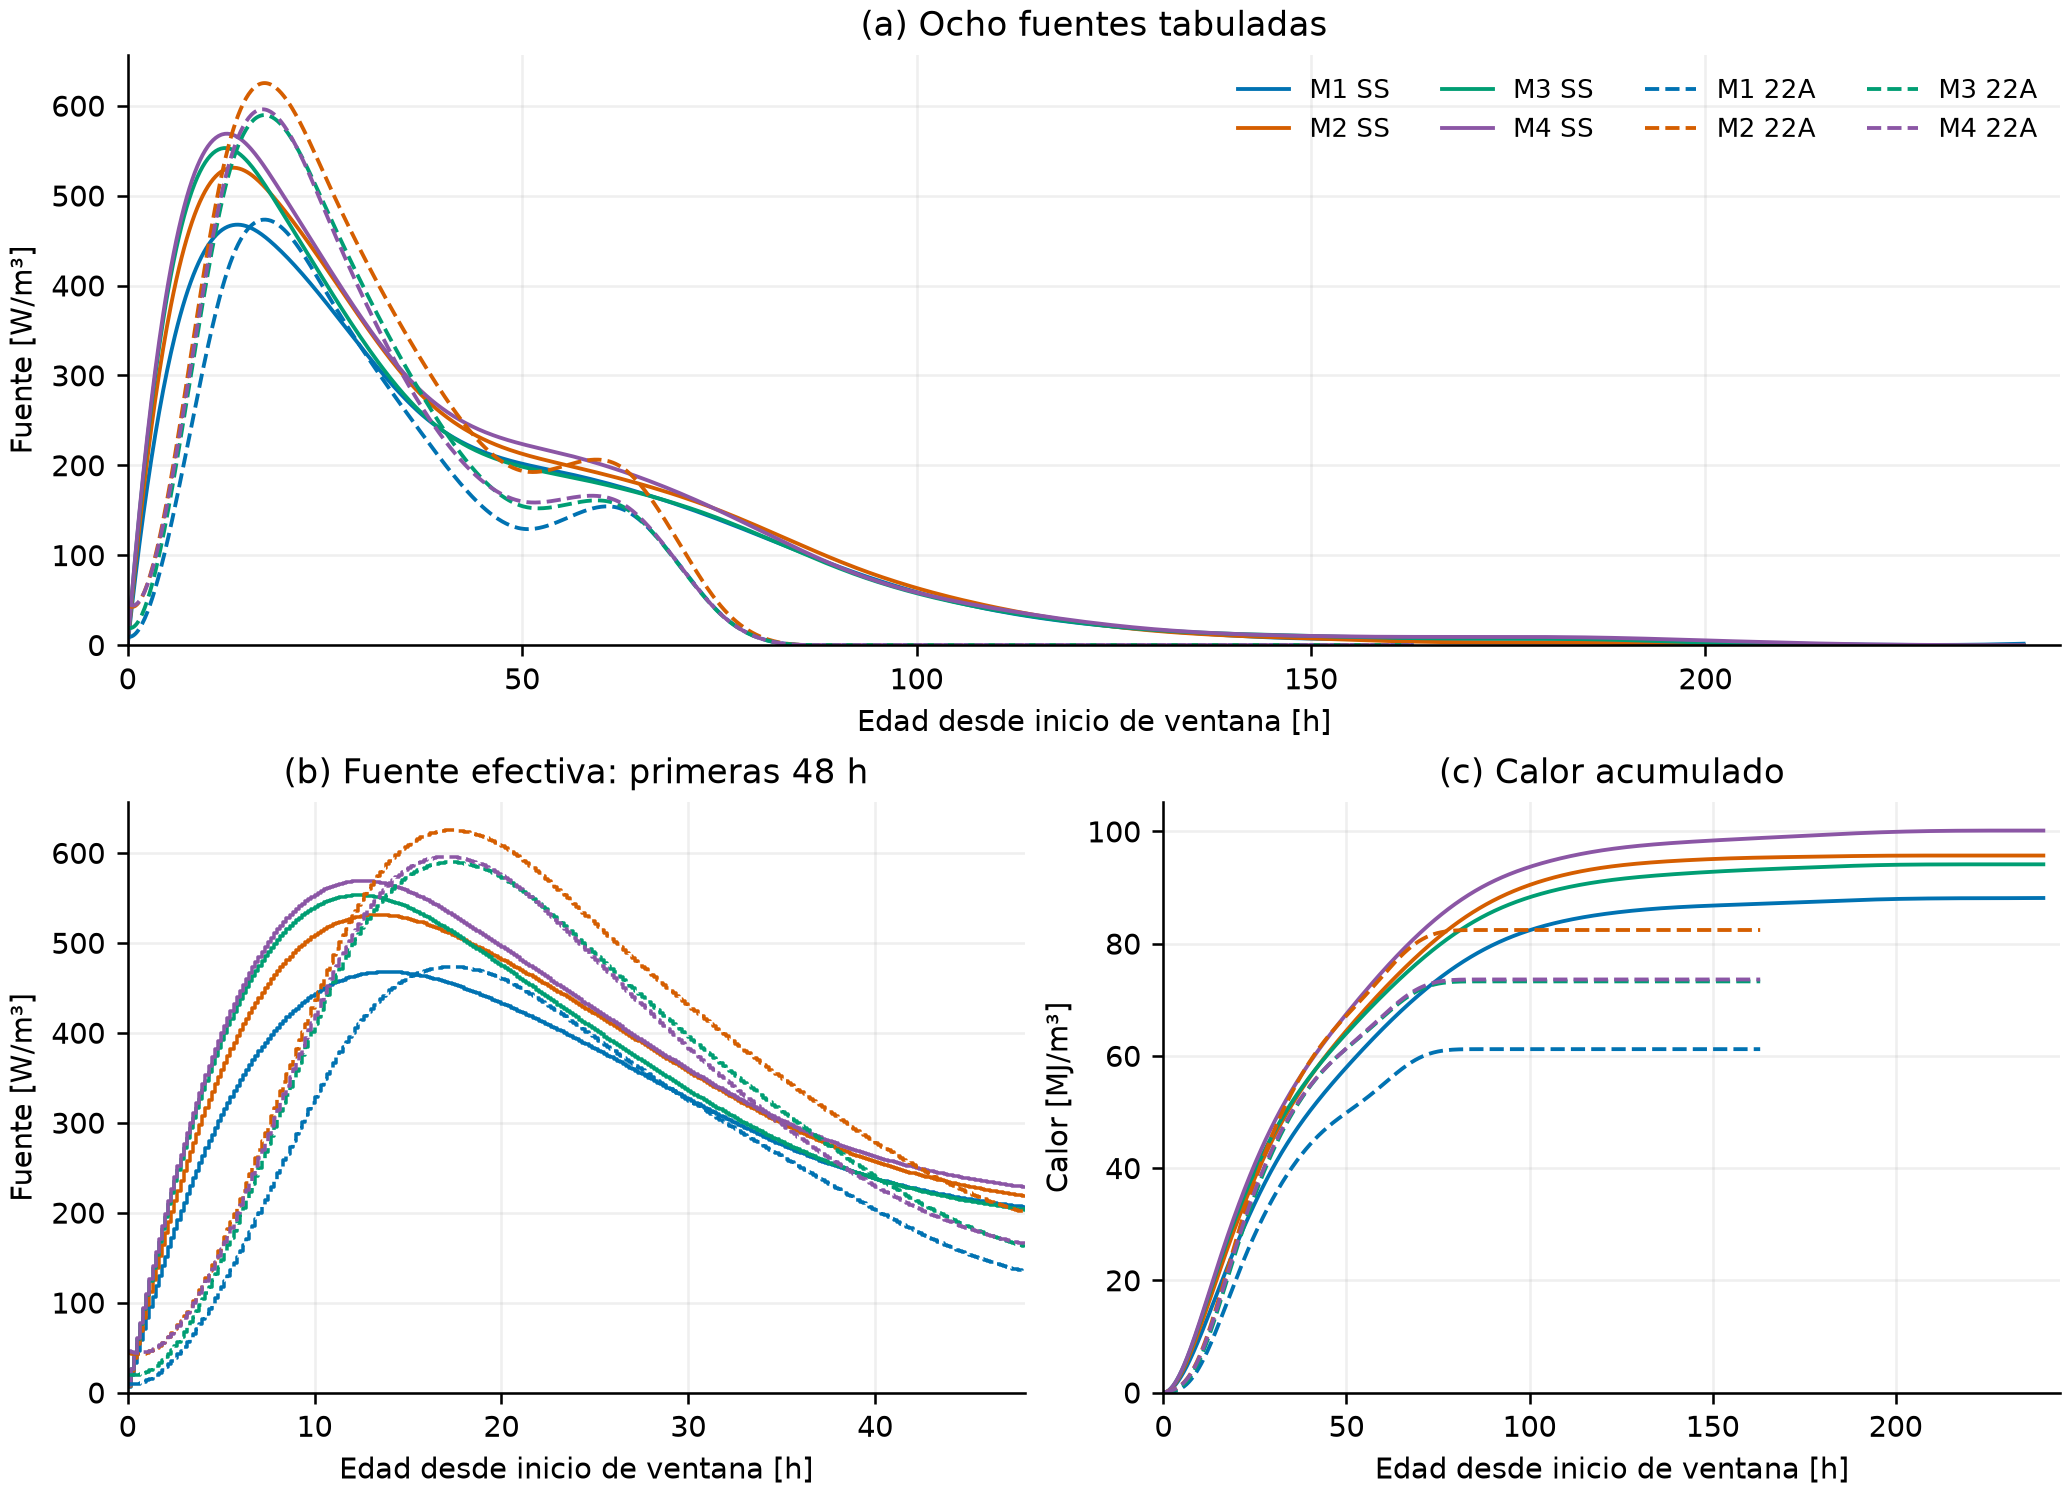
\includegraphics[width=0.98\linewidth]{Imagenes/hidratacion_fuentes_calor.png}
  \caption{Fuentes tabuladas, fuente efectiva y calor acumulado de las ocho curvas de hidratación}
  \label{fig:hidratacion-fuentes}
  \captionsetup{skip=2pt}
  \caption*{Fuente: Elaboración propia a partir de \texttt{source\_terms.txt} y de los archivos tabulares del modelo.}
\end{figure}


%-------------------------------------------
\subsection{Datos meteorológicos y tratamiento temporal}
\label{sec:Meteorologicos}
%-------------------------------------------

El clima se representa mediante tres historias horarias de los años $2023$, $2024$ y $2025$, obtenidas de ERA5 a través de la API histórica de Open-Meteo \citep{openmeteoHistorico}. ERA5 es un reanálisis: combina observaciones y un modelo atmosférico para reconstruir las condiciones del pasado. Por ello, estas series se utilizan como escenarios históricos del sitio y no como pronósticos del tiempo que ocurriría durante la construcción en $2026$.

Las consultas utilizan las coordenadas del apartado~\ref{sec:emplazamiento-geometria}. La respuesta del proveedor corresponde al punto de grilla de latitud $-37{,}25^{\circ}$ y longitud $-72{,}25^{\circ}$. Esta diferencia refleja la representación espacial del producto; los valores no son mediciones tomadas en la posición exacta de la fundación. Las solicitudes conservadas permiten identificar tanto las coordenadas pedidas como las devueltas.
\newpage

Cada archivo abarca del $19$ de noviembre al $17$ de diciembre de su año, desde las $00{:}00$ del primer día hasta las $23{:}00$ del último, en UTC, con $696$ marcas horarias. Los datos iniciales incluyen temperatura del aire, viento y radiación global. Posteriormente se descargaron archivos complementarios para incorporar las variables necesarias para radiación, sin reemplazar los anteriores. La Tabla~\ref{tab:descargas-clima} identifica ambas descargas; los instantes se muestran hasta el segundo, y los metadatos conservan su precisión original.

\begin{table}[htbp]
  \centering
  \caption{Descargas de las historias meteorológicas utilizadas}
  \label{tab:descargas-clima}
  \small
  \begin{tabular}{lcc}
    \toprule
    Historia & Descarga inicial [UTC] & Descarga complementaria [UTC] \\
    \midrule
    ERA5-$2023$ & $17/11/2026$, $01{:}37{:}07$ & $18/11/2026$, $20{:}02{:}51$ \\
    ERA5-$2024$ & $17/11/2026$, $01{:}37{:}06$ & $18/11/2026$, $20{:}02{:}53$ \\
    ERA5-$2025$ & $17/11/2026$, $01{:}37{:}07$ & $18/11/2026$, $20{:}02{:}54$ \\
    \bottomrule
  \end{tabular}
  \captionsetup{skip=2pt}
  \caption*{Fuente: metadatos de los archivos descargados de Open-Meteo.}
\end{table}

Para relacionar cada historia con la obra, se toma el $19$ de noviembre de su año a las $10{:}00$, UTC$-03{:}00$, como inicio de tiempo relativo. Esa hora corresponde a las $13{:}00$ UTC. A partir de ella se conserva la secuencia horaria completa y se aplica al inicio constructivo del $19$ de noviembre de $2026$, declarado en el apartado anterior. Así se mantienen los ciclos diarios y la relación entre las variables de cada historia. La posición solar se calcula con las fechas históricas correspondientes. Los archivos se almacenan en UTC y el inicio de obra se identifica con la zona \texttt{America/Santiago}, evitando confundir ambas referencias.

La Tabla~\ref{tab:variables-clima} resume las variables que intervienen en los intercambios térmicos. La temperatura del aire, el viento y la radiación global de las descargas complementarias coinciden exactamente con los archivos iniciales en las tres historias. La radiación directa horizontal también se conserva para comprobar su suma con la difusa frente a la global. La temperatura del cielo se estima a partir del punto de rocío y la nubosidad total; no se dispone de una medición infrarroja del cielo. El suelo mantiene el tratamiento equivalente descrito en el apartado~\ref{sec:Parametros y condiciones}, sin utilizar una serie de temperatura del terreno.

\begin{table}[htbp]
  \centering
  \caption{Variables meteorológicas y uso en el modelo térmico}
  \label{tab:variables-clima}
  \small
  \setlength{\tabcolsep}{4pt}
  \begin{tabular}{p{5.0cm}p{1.8cm}p{9.0cm}}
    \toprule
    Variable & Unidad & Uso \\
    \midrule
    Temperatura del aire a $2\,\mathrm{m}$ & $^{\circ}\mathrm{C}$ & Intercambio convectivo y cálculo del entorno radiativo \\
    Velocidad del viento a $10\,\mathrm{m}$ & $\mathrm{m\,s^{-1}}$ & Ajuste a $2\,\mathrm{m}$ y cálculo del coeficiente convectivo \\
    Radiación global horizontal (GHI) & $\mathrm{W\,m^{-2}}$ & Radiación sobre caras superiores y reflexión del entorno \\
    Radiación directa normal (DNI) & $\mathrm{W\,m^{-2}}$ & Componente directa según la orientación de cada cara \\
    Radiación difusa horizontal (DHI) & $\mathrm{W\,m^{-2}}$ & Componente difusa sobre las caras expuestas \\
    Punto de rocío a $2\,\mathrm{m}$ & $^{\circ}\mathrm{C}$ & Estimación de la emisión térmica del cielo \\
    Nubosidad total & $\%$ & Aproximación de la nubosidad opaca en la estimación del cielo \\
    \bottomrule
  \end{tabular}
  \captionsetup{skip=2pt}
  \caption*{Fuente: Archivos meteorológicos y tratamiento implementado en el modelo.}
\end{table}
\newpage

Entre las marcas horarias se interpola linealmente la temperatura del aire, el punto de rocío y la nubosidad. El coeficiente convectivo se mantiene constante durante cada hora, calculado con el viento de su marca inicial. Las irradiancias representan el promedio de la hora precedente \citep{openmeteoHistorico}: para el intervalo entre dos marcas se utiliza el dato de la marca final, con la posición solar evaluada en el punto medio. Este tratamiento respeta el intervalo temporal al que pertenece la energía solar.

Las Figuras~\ref{fig:clima-ambiente} y~\ref{fig:clima-radiacion} muestran las series utilizadas durante las $672\,\mathrm{h}$ y el coeficiente convectivo calculado. La línea vertical en $336\,\mathrm{h}$ distingue el horizonte obligatorio del seguimiento extendido. Se verificó la continuidad horaria y la ausencia de valores faltantes en las variables utilizadas. La cobertura disponible permite completar ambos horizontes sin repetir días, rellenar huecos ni prolongar la última temperatura. Las diferencias entre estas tres historias representan parte de la variación climática posible; su número limitado no permite tratarlas como una descripción completa de los extremos meteorológicos del sitio.

\begin{figure}[htbp]
  \centering
  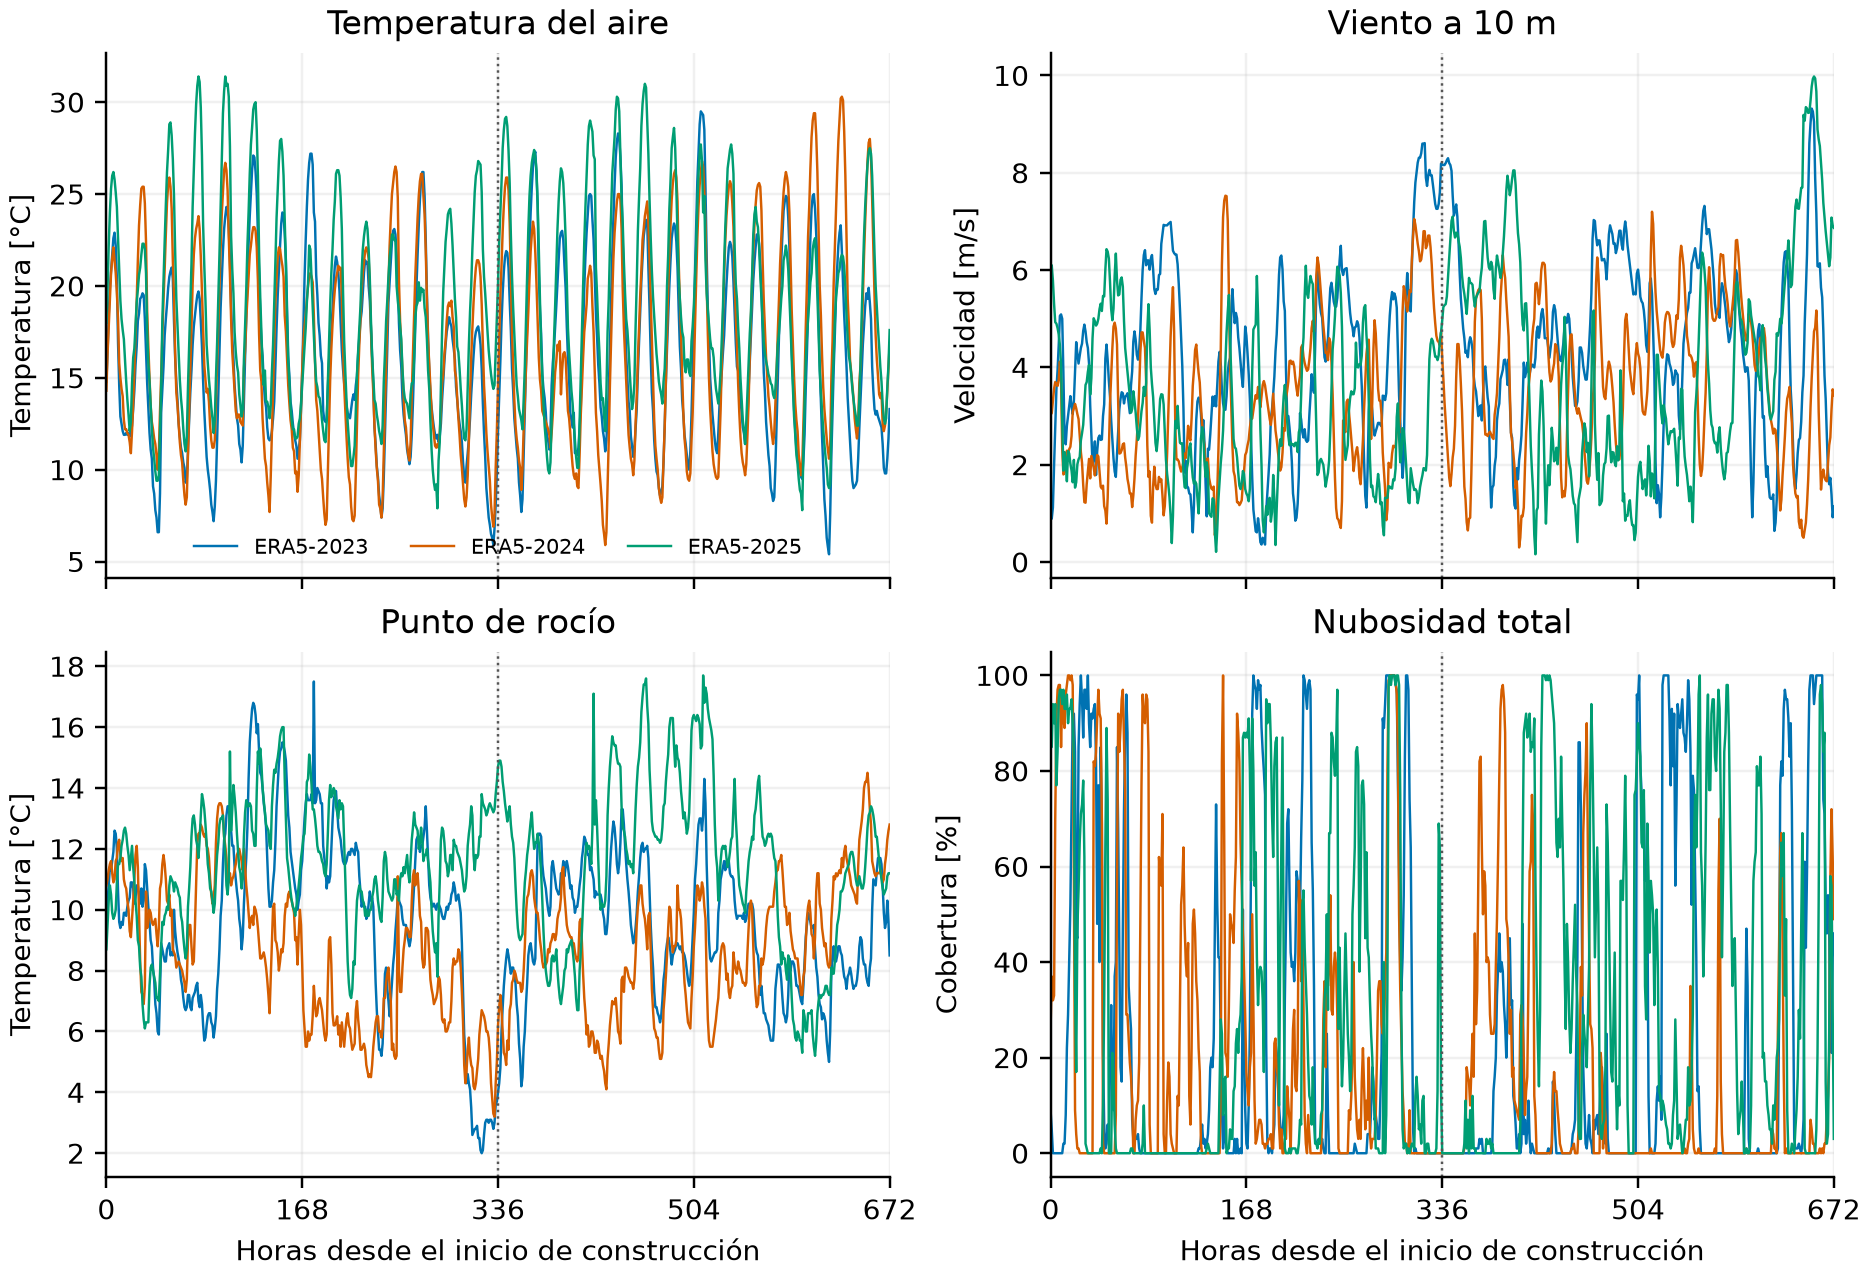
\includegraphics[width=0.95\linewidth]{Imagenes/clima_ambiente.png}
  \caption{Temperatura del aire, viento, punto de rocío y nubosidad de las tres historias climáticas}
  \label{fig:clima-ambiente}
  \captionsetup{skip=2pt}
  \caption*{Fuente: Elaboración propia a partir de los archivos ERA5 descargados de Open-Meteo.}
\end{figure}
\newpage
\begin{figure}[h]
  \centering
  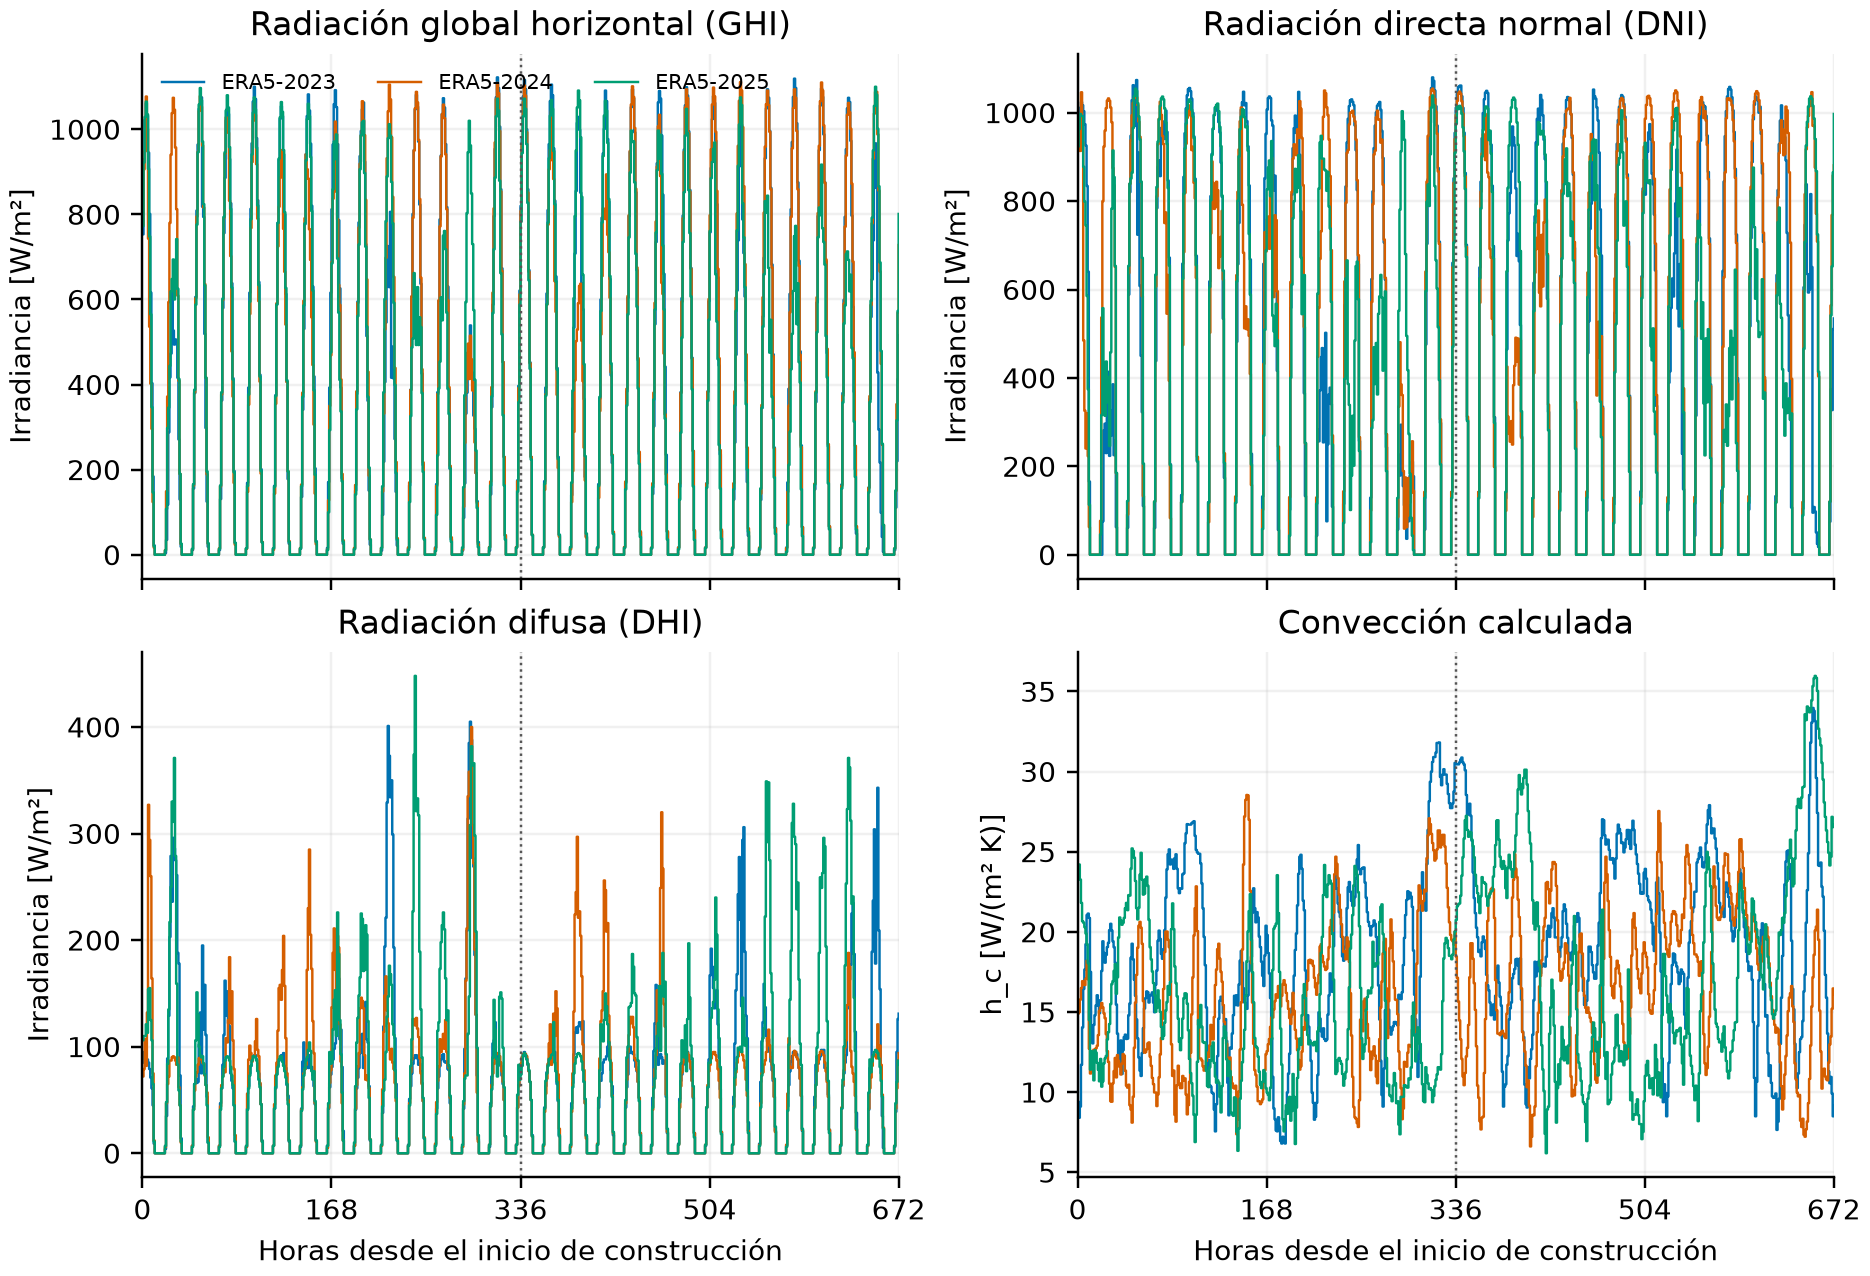
\includegraphics[width=0.95\linewidth]{Imagenes/clima_radiacion_conveccion.png}
  \caption{Radiación solar y coeficiente convectivo utilizados en las tres historias climáticas}
  \label{fig:clima-radiacion}
  \captionsetup{skip=2pt}
  \caption*{Fuente: Elaboración propia a partir de los archivos ERA5 y de la correlación convectiva adoptada.}
\end{figure}

En ambas figuras, el eje horizontal representa las horas transcurridas desde el inicio de construcción y los colores distinguen las tres historias climáticas. Los ejes verticales indican la variable representada y su unidad.

La Figura~\ref{fig:clima-ambiente} muestra los ciclos diarios de temperatura y las diferencias de viento, punto de rocío y nubosidad entre las historias. En la Figura~\ref{fig:clima-radiacion} se observa la alternancia de la radiación solar entre el día y la noche, mientras que el coeficiente convectivo cambia con la velocidad del viento. Estas variaciones hacen que las condiciones de intercambio de calor entre la fundación y el ambiente cambien durante el seguimiento.

%-------------------------------------------
\subsection{Trazabilidad y congelación de los datos}
\label{sec:Trazabilidad}
%-------------------------------------------

La comparación utiliza copias locales de los datos, conservadas sin cambios durante la campaña de cálculo. Cada archivo meteorológico guarda la respuesta original del proveedor y los metadatos de la consulta: dirección de acceso, variables, coordenadas, unidades, zona horaria y fecha de descarga. El manifiesto de radiación vincula cada archivo complementario con su descarga inicial y registra la coincidencia de las variables comunes. Esto permite reconstruir qué información se utilizó sin depender de una nueva consulta al servicio.

\newpage
El repositorio conserva las descargas históricas en \path{datos/clima/reanalisis}, las complementarias en \path{datos/clima/radiacion} y los pronósticos previos en \path{datos/clima/forecasts}. Entre estos últimos existen archivos descargados el $10$ y el $17$ de noviembre de $2026$. Se mantienen como antecedentes de las etapas anteriores; la comparación final de este artículo se basa en las tres historias ERA5 descritas, sin mezclarlas con esos pronósticos. La ampliación de variables del $18$ de noviembre corresponde a una descarga efectivamente registrada, no a una reconstrucción retrospectiva de información supuestamente disponible antes.

La configuración final identifica el IFC, las curvas de hidratación, los planes y las condiciones térmicas. Los resultados por escenario registran esas referencias junto con huellas SHA-256, códigos que permiten comprobar si un archivo ha cambiado. Se contrastaron las referencias climáticas de las $72$ corridas archivadas del cierre: las dos tasas de colocación y la confirmación fina de la propuesta utilizan los mismos datos meteorológicos para cada historia. De esta forma, la comparación no obtiene ventajas por cambiar el clima entre planes o resoluciones.

Para facilitar la revisión del artículo, se archivaron las series mostradas en las figuras, los metadatos y las huellas de los insumos en \path{entregas/F01/articulo/datos}. Las configuraciones y métricas completas permanecen en sus carpetas de origen. Cualquier corrección posterior a la defensa debe conservar la versión previa y registrar qué cambió, por qué y si modifica la recomendación. Los identificadores de los commits de defensa y de entrega final se documentarán junto con los comandos de reproducción en el anexo correspondiente; las huellas de archivos no sustituyen esos identificadores.

\section{Modelo continuo}
\label{sec:modelo-continuo}

\subsection{Dominio y supuestos físicos}
La fundación crece durante la colocación. Si $\Omega_j$ representa la capa $j$ y $t_j$ su instante de activación, el dominio de conducción y la edad local se expresan como
\begin{equation}
  \Omega_c(t)=\bigcup_{j:\,t\geq t_j}\Omega_j,
  \qquad a_j(t)=t-t_j.
  \label{eq:dominio-edad}
\end{equation}
Solo el hormigón colocado almacena y conduce calor. Su densidad $\rho$, su calor específico $c_p$ y su conductividad $k_c$ se suponen constantes e iguales en todas las capas. Esta elección permite aislar el efecto del cronograma con las propiedades disponibles. El terreno, el moldaje y el agua se representan por sus intercambios con el hormigón.

\subsection{Balance local de energía y conducción}
En un volumen fijo $V$ de hormigón activo, el cambio de energía sensible es igual al calor que atraviesa el contorno más el generado por hidratación y menos el retirado por los circuitos \citep{inlTransferencia}. Con normal saliente $\vec n$, flujo conductivo $\vec q$ en $\mathrm{W\,m^{-2}}$ y temperatura de referencia constante $T_{\mathrm{ref}}$, el balance y la ley de Fourier son
\begin{equation}
  \frac{d}{dt}\int_V \rho c_p(T-T_{\mathrm{ref}})\,dV
  =-\int_{\partial V}\vec{q}\cdot\vec{n}\,dA
   +\int_V(\dot q_h-\dot q_r)\,dV.
  \label{eq:balance-integral}
\end{equation}
\begin{equation}
  \vec{q}=-k_c\vec{\nabla} T.
  \label{eq:fourier}
\end{equation}
Al aplicar el teorema de la divergencia al flujo y considerar un volumen arbitrario se obtiene la ecuación que se resuelve dentro del hormigón:
\begin{equation}
  \rho c_p\frac{\partial T}{\partial t}
  =\vec{\nabla}\cdot(k_c\vec{\nabla} T)+\dot q_h-\dot q_r,
  \qquad \vec{x}\in\Omega_c(t).
  \label{eq:calor-modelo}
\end{equation}
Los términos $\dot q_h$ y $\dot q_r$ expresan potencia por unidad de volumen, en $\mathrm{W\,m^{-3}}$. El primero calienta el material y el segundo retira energía cuando el sistema de refrigeración lo permite.

\subsection{Colocación, condiciones iniciales e hidratación}
Para una tasa constante $q$ y sin esperas, cada capa de volumen $V_j$ tarda $V_j/q$ en colocarse. El modelo activa todo su volumen al comienzo de ese intervalo. El hormigón ya colocado conserva su temperatura y el nuevo entra con la condición
\begin{equation}
  T(\vec{x},t_j^+)=T_{\mathrm{col}}=12\,^{\circ}\mathrm{C},
  \qquad \vec{x}\in\Omega_j.
  \label{eq:inicial-colocacion}
\end{equation}
Todas las capas de un escenario utilizan la misma curva $m$, desplazada según su edad local. La fuente efectiva se obtiene del calor acumulado en la sección anterior:
\begin{equation}
  \dot q_h(\vec{x},t)=\frac{dH_m}{da}\bigl(a_j(t)\bigr),
  \qquad \vec{x}\in\Omega_j,\quad t\geq t_j.
  \label{eq:fuente-edad}
\end{equation}
La velocidad de hidratación depende solo de la edad. En un ensayo adiabático bastaría multiplicar la tasa de aumento de temperatura por $\rho c_p$. Las probetas docentes pierden calor por su superficie. El balance empleado para interpretar la inversión incluye también esa pérdida:
\begin{equation}
  \dot q_m(t)=\frac{1}{V_p}\frac{d}{dt}
       \int_{V_p}\rho c_p(T_p-T_{\mathrm{ref}})\,dV
       +\frac{1}{V_p}\int_{\partial V_p}\beta_p(T_{p,s}-T_a)\,dA.
  \label{eq:balance-probeta}
\end{equation}
Aquí $V_p$ es el volumen de la probeta, $T_p$ su temperatura interior, $T_{p,s}$ su temperatura superficial y $T_a$ la del aire. La conductancia $\beta_p=2{,}5\,\mathrm{W\,m^{-2}\,K^{-1}}$ corresponde al ajuste docente. El modelo de la fundación recibe el resultado de ese ajuste.

\subsection{Refrigeración equivalente y control}
La refrigeración actúa únicamente en la región de cada circuito abierto. La extracción aumenta con el exceso de temperatura del hormigón sobre el agua, que se supone uniforme a $T_w=18\,^\circ\mathrm C$:
\begin{equation}\begin{aligned}
  \dot q_r^0(\vec{x},t)&=U_v\sum_{b=1}^{9}
       \chi_b(\vec{x})\,s_b(t)\max(T-T_w,0),\\
  P_r^0(t)&=\int_{\Omega_c(t)}\dot q_r^0\,dV,
  \qquad \dot q_r=\lambda(t)\dot q_r^0,
  \end{aligned}\label{eq:extraccion-equivalente}\end{equation}
La función $\chi_b$ identifica la región del ramal $b$ y $s_b$ vale uno si está abierto. El coeficiente volumétrico $U_v$ se fija en $5\,\mathrm{W\,m^{-3}\,K^{-1}}$. Si la potencia solicitada $P_r^0$ supera $15\,\mathrm{kW}$, se reducen todos los aportes en la misma proporción mediante $\lambda=P_{\max}/P_r^0$; en los demás casos $\lambda=1$.

Cada circuito comienza cerrado. Una vez cubierto, abre cuando el punto más frío de sus controles alcanza $19\,^\circ\mathrm C$ y cierra cuando baja a $18\,^\circ\mathrm C$ o menos. La ley representa la capacidad de extracción adoptada. Determinar si el montaje la alcanza exige comprobar la transferencia real, la hidráulica y el calentamiento del agua a lo largo del ramal.

\subsection{Superficies expuestas y protecciones}
La madera y las mantas se representan como resistencias en serie. El calor entrante $\phi=-\vec q\cdot\vec n$ es positivo hacia el hormigón. Entre la cara del hormigón a $T_b$ y el exterior de la protección a $T_s$ se cumple
\begin{equation}
  R_p(a)=\sum_{\ell\,\mathrm{instalada}}\frac{e_\ell}{k_\ell},
  \qquad T_s-T_b=R_p(a)\,\phi,
  \label{eq:resistencia-proteccion}
\end{equation}
Los espesores $e_\ell$ y las conductividades $k_\ell$ corresponden a las capas instaladas en ese instante. Se supone despreciable su almacenamiento de calor y la resistencia de sus contactos. Si solo hubiera convección, se obtendría el coeficiente equivalente
\begin{equation}
  -k_c\vec{\nabla} T\cdot\vec{n}=h_{\mathrm{eq}}(T_b-T_a),
  \qquad h_{\mathrm{eq}}^{-1}=h_c^{-1}+R_p.
  \label{eq:robin-equivalente}
\end{equation}
En el cálculo se resuelve además el intercambio radiativo en la cara exterior. Al retirar una protección se elimina su resistencia. Cuando se retira la última, $T_s=T_b$.

\subsection{Radiación solar y de onda larga}
La cara exterior comparte calor con el aire, absorbe radiación solar y emite radiación de onda larga hacia el cielo y el entorno \citep{energyplusMcAdams}. Su balance por unidad de superficie es
\begin{equation}
  \phi=\mathcal F(T_s)
  =h_c(T_a-T_s)+\alpha_{\mathrm{SW}}I_f
   +\varepsilon\sigma\left[
      F_{\mathrm{sky}}T_{\mathrm{sky},K}^{4}
      +(1-F_{\mathrm{sky}})T_{a,K}^{4}-T_{s,K}^{4}\right].
  \label{eq:balance-exterior}
\end{equation}
$T_a$ representa la temperatura del aire, $I_f$ la irradiancia que recibe la cara y $T_{\mathrm{sky},K}$ la temperatura radiativa del cielo. El viento determina $h_c$, mientras que $\alpha_{\mathrm{SW}}$, $\varepsilon$ y $\sigma$ son la absortancia, la emisividad y la constante de Stefan--Boltzmann. Las temperaturas elevadas a la cuarta potencia se expresan en kelvin. El factor de vista $F_{\mathrm{sky}}$ vale $1$ arriba, $0{,}5$ en caras verticales y $0$ abajo. La temperatura efectiva del cielo se estima con el punto de rocío y la nubosidad, mediante las relaciones de Clark--Allen y Walton \citep{energyplusCielo}.

El eje $+x$ apunta al este y el eje $+y$ al norte. Las caras superiores reciben la irradiancia global horizontal. En las verticales se suman la radiación directa proyectada sobre la normal, la mitad de la difusa y la mitad de la global reflejada por el terreno con albedo $0{,}20$. Las inferiores expuestas reciben solo la componente reflejada. La posición del sol se calcula a mitad de cada hora histórica \citep{noaaSolar}. Desde la edad local de $504\,\mathrm h$, la sombra multiplica la irradiancia por $0{,}10$ y conserva la convección y la onda larga.

\subsection{Suelo, interfaces y cambios de borde}
La base conduce calor a través de una resistencia equivalente $R_g=L_g/k_g$ hacia un reservorio que permanece a $T_g=15\,^\circ\mathrm C$ desde el inicio. El modelo omite la evolución térmica del suelo. Entre capas activas se supone contacto perfecto, con una misma normal $\vec n_j$ para comparar los flujos a ambos lados:
\begin{equation}
  -k_c\vec{\nabla} T\cdot\vec{n}=\frac{T_b-T_g}{R_g}.
  \label{eq:borde-suelo}
\end{equation}
\begin{equation}
  T^-=T^+,\qquad
  -k^-\vec{\nabla} T^-\cdot\vec{n}_j
  =-k^+\vec{\nabla} T^+\cdot\vec{n}_j.
  \label{eq:contacto-capas}
\end{equation}
Cuando una capa nueva cubre una cara, el intercambio con el aire cesa y comienza la conducción hacia la capa vecina. La Tabla~\ref{tab:bordes-etapas} reúne las condiciones aplicadas ($R_m=e_m/k_m$ para la madera y $R_a=e_a/k_a$ para cada manta), incluidas las etapas durante las cuales la madera o las mantas siguen protegiendo cada superficie.
\begin{table}[htbp]
  \centering
  \caption{Condiciones de borde e interfaces por superficie y etapa}
  \label{tab:bordes-etapas}
  \small
  \setlength{\tabcolsep}{3pt}
  \begin{tabular}{L{2.5cm}L{2.0cm}L{3.7cm}L{3.0cm}L{4.5cm}}
    \toprule
    Superficie & Etapa & Ecuación & Parámetros & Fuente y fundamento \\
    \midrule
    Lateral al aire & $0\leq a<72\,\mathrm h$ & $\phi=\mathcal F(T_s)$ & $R_p=R_m+2R_a$ & AraucoPly, Aislanglass y plan: madera con dos mantas \\
    Lateral al aire & $72\leq a<240\,\mathrm h$ & $\phi=\mathcal F(T_s)$ & $R_p=2R_a$ & Plan: retiro de madera y conservación de mantas \\
    Superior al aire & $0\leq a<240\,\mathrm h$ & $\phi=\mathcal F(T_s)$ & $R_p=2R_a$ & Aislanglass y plan: dos mantas, sin madera \\
    Lateral o superior al aire & $240\leq a<504\,\mathrm h$ & $\phi=\mathcal F(T_s)$ & $R_p=R_a$ & Plan: retiro de la primera manta \\
    Lateral o superior al aire & $a\geq504\,\mathrm h$ & $\phi=\mathcal F(T_b)$ con $I_f$ atenuada & $R_p=0$, $\tau=0{,}10$ & Plan: retiro de última manta y sombra idealizada \\
    Base sobre suelo & Desde su activación & $\phi=(T_g-T_b)/R_g$ & $T_g=15\,^{\circ}\mathrm C$, $R_g=L_g/k_g$ & Supuesto de reservorio y conducción equivalente \\
    Interfaz interna & Ambas capas activas & $T^-=T^+$ y continuidad de flujo, Ec.~\eqref{eq:contacto-capas} & Resistencia de junta nula & Contacto perfecto supuesto, sin borde de aire \\
    \bottomrule
  \end{tabular}
  \captionsetup{skip=2pt}
  \caption*{Fuente: configuración final del estudio, referencias de materiales y ecuaciones del modelo implementado.}
\end{table}

\section{Discretización y algoritmos}
\label{sec:discretizacion}

\subsection{Balance de energía por celda}
Cada celda activa tiene volumen $V_i=h^3$, caras de área $A_f=h^2$ y distancia $d_i=h/2$ desde el centro a una cara. Al integrar la ecuación de energía en ese volumen y aplicar el teorema de la divergencia, el término conductivo queda expresado como una suma de flujos por caras:
\begin{equation}
  \frac{d}{dt}\int_{V_i}\rho c_pT\,dV
  =\sum_{f\subset\partial V_i}\int_{A_f}
  k\vec{\nabla}T\cdot\vec{n}_{i,f}\,dA
  +\int_{V_i}\dot q_h\,dV-P_{r,i}.
  \label{eq:balance-integral-celda}
\end{equation}
Al aproximar cada flujo por su valor en la cara y la temperatura por el valor del centro, se obtiene
\begin{equation}
  C_i\frac{dT_i}{dt}
  =\sum_{j\in\mathcal N_i}G_{ij}(T_j-T_i)
   +\dot q_{h,i}V_i+Q_{b,i}-P_{r,i},
  \qquad C_i=\rho_i c_{p,i}V_i.
  \label{eq:balance-celda}
\end{equation}
Aquí $\mathcal N_i$ reúne las celdas activas que comparten una cara con $i$. La capacidad $C_i$ se expresa en $\mathrm{J\,K^{-1}}$, la conductancia $G_{ij}$ en $\mathrm{W\,K^{-1}}$, y las potencias de borde entrante $Q_{b,i}$ y de refrigeración $P_{r,i}$ en vatios. Las resistencias de las dos medias celdas se suman en serie:
\begin{equation}
  G_{ij}=\frac{A_{ij}}{d_i/k_i+d_j/k_j}.
  \label{eq:conductancia-vecinos}
\end{equation}
La potencia de borde suma $A_f\phi_f$ sobre las caras exteriores de la celda. En el suelo, la resistencia por unidad de área es $d_i/k_c+L_g/k_g$; en el aire, la resistencia entre el centro y la superficie exterior es $R_{i,f}=d_i/k_c+R_p$. Una cara compartida por dos celdas activas aporta potencias de igual magnitud y signo contrario.

\subsection{Avance temporal y balance radiativo}
El avance explícito de Euler evalúa los intercambios con las temperaturas conocidas al comienzo del paso. Para la hidratación se utiliza directamente el incremento del calor acumulado, que conserva el aporte aun cuando el paso no coincida con el intervalo de las muestras:
\begin{equation}
  T_i^{n+1}=T_i^n+\frac{1}{C_i}\Bigl\{\Delta t_n\Bigl[\sum_{j\in\mathcal N_i}G_{ij}(T_j^n-T_i^n)+Q_{b,i}^n-P_{r,i}^n\Bigr]+V_i\bigl[H_m(a_i^{n+1})-H_m(a_i^n)\bigr]\Bigr\}.
  \label{eq:euler-fundacion}
\end{equation}
En cada cara expuesta se obtiene $T_s$ igualando $(T_s-T_i^n)/R_{i,f}$ con el flujo exterior del balance radiativo. Se emplea Newton con un máximo de nueve iteraciones, una corrección inferior a $10^{-10}\,\mathrm K$ y una comprobación del residuo de $2\times10^{-8}\,\mathrm{W\,m^{-2}}$. La extracción de cada celda se limita a la energía disponible sobre $T_w$ durante el paso antes de aplicar el tope conjunto. El avance del hormigón sigue siendo explícito.

\subsection{Selección del paso y estabilidad}
Para que los coeficientes de una actualización lineal con conductancias positivas sean no negativos, la capacidad de cada celda y su conductancia total de borde $G_{b,i}$ imponen
\begin{equation}
  \Delta t\leq
  \frac{C_i}{\displaystyle\sum_{j\in\mathcal N_i}G_{ij}+G_{b,i}},
  \label{eq:limite-lineal}
\end{equation}
En el problema con radiación, la suma conservadora $S_i$ incluye las conductancias entre vecinos, $A_f/R_{i,f}$ en las caras al aire, las conductancias hacia el suelo y $U_vV_i$ en las celdas refrigerables. El término de aire acota la variación del flujo no lineal respecto de la temperatura interior. El cálculo aplica el siguiente paso:
\begin{equation}
  \Delta t_n=\min\left(
     \Delta t_{\max},\;
     0{,}8\min_{i:S_i>0}\frac{C_i}{S_i},\;
     t_{\mathrm{evento}}-t_n\right).
  \label{eq:paso-utilizado}
\end{equation}
El factor $0{,}8$ deja margen y el último término hace coincidir el avance con activaciones, retiros, cambios horarios y fin del horizonte. La apertura y el cierre se evalúan en los pasos. La restricción de estabilidad se complementó con un contraste temporal para comprobar cuánto cambian los resultados.

\subsection{Temperatura superficial y extracción a \texorpdfstring{$25\,\mathrm{mm}$}{25 mm}}
La primera celda tiene su centro a más de $25\,\mathrm{mm}$ del contorno en ambas mallas. Para estimar la temperatura a esa profundidad se reconstruye un perfil lineal a partir del flujo entrante en cada cara exterior, incluida la base:
\begin{equation}
  T_{b,f}=T_i+\phi_f\frac{d_i}{k_c},
  \qquad
  T_{25,f}=T_i+\phi_f\frac{d_i-\delta}{k_c},
  \qquad \delta=0{,}025\,\mathrm m.
  \label{eq:reconstruccion-s25}
\end{equation}
El desplazamiento $\delta$ sigue la normal interior de la cara cartesiana. Las caras escalonadas explican por qué la posición reconstruida es aproximada en los contornos inclinados. En cada instante se comparan centros y caras para obtener el máximo, y se busca el mínimo entre todos los puntos reconstruidos a $\delta$. El diferencial utiliza ambas temperaturas simultáneas.

\subsection{Resoluciones y sensibilidad de la discretización}
Las dos tasas se compararon con $h=0{,}40\,\mathrm m$ y paso máximo de $300\,\mathrm s$. Para aislar el efecto espacial se refinó la malla de la propuesta manteniendo el origen, las once capas, el paso y la zona refrigerable. En el contraste temporal se mantuvo la malla base y se redujo el paso máximo a la mitad. La Tabla~\ref{tab:contrastes-discretizacion} indica cuántos escenarios cubrió cada prueba.
\begin{table}[htbp]
  \centering
  \caption{Contrastes de sensibilidad utilizados para evaluar la discretización}
  \label{tab:contrastes-discretizacion}
  \small
  \setlength{\tabcolsep}{4pt}
  \begin{tabular}{L{2.0cm}L{3.6cm}L{3.8cm}L{2.5cm}L{2.5cm}}
    \toprule
    Contraste & Configuraciones & Escenarios & Mayor cambio de $T_{\max}$ [K] & Mayor cambio de $\Delta T_{\max}$ [K] \\
    \midrule
    Espacial & $0{,}40\to0{,}20\,\mathrm m$; $300\,\mathrm s$ & $24$ pares de la propuesta & $0{,}669459$ & $0{,}881712$ \\
    Temporal & $300\to150\,\mathrm s$; $0{,}40\,\mathrm m$ & \texttt{M4\_SS} con ERA5-$2024$ y ERA5-$2025$ & $0{,}001148$ & $0{,}001365$ \\
    \bottomrule
  \end{tabular}
  \captionsetup{skip=2pt}
  \caption*{Fuente: elaboración propia a partir de las simulaciones con ambas resoluciones.}
\end{table}

\subsection{Secuencia del algoritmo}
Para seguir una realización basta escoger un plan, una curva y una historia meteorológica. La secuencia se repite con las mismas reglas para todas las combinaciones:
\begin{enumerate}
\item Leer la geometría, preparar la malla y asignar a cada celda su capa y su zona de refrigeración. Cargar el cronograma, las propiedades y los datos del escenario.
\item Comenzar con los circuitos cerrados. Al llegar al inicio de una capa, incorporarla a su temperatura de colocación y actualizar las caras que pasan del aire al contacto con hormigón.
\item Revisar las protecciones según la edad local, calcular el paso admisible y obtener la energía de hidratación generada entre sus dos extremos.
\item Resolver el intercambio de cada cara, comprobar el estado de los circuitos y avanzar simultáneamente las temperaturas. Registrar la energía que entra, sale y queda almacenada.
\item Buscar extremos durante el avance y a ambos lados de los cambios de borde. Guardar sus posiciones e instantes hasta completar el seguimiento.
\item Repetir para los escenarios restantes. Sumar los pesos de los que exceden algún umbral y comparar los planes por su duración y cumplimiento.
\end{enumerate}

\subsection{Equipo y costo computacional}
El equipo identificado al preparar el artículo utilizaba Windows $10$, un Intel Core i7-10750H y $12$ procesadores lógicos. Los tiempos de la Tabla~\ref{tab:tiempos-corridas} proceden de los registros de cada ejecución, también cuando se recuperó un cálculo anterior. La mediana de una simulación fina fue de aproximadamente $12\,\mathrm{min}$.
\begin{table}[htbp]
  \centering
  \caption{Duraciones registradas de las corridas a $672\,\mathrm h$}
  \label{tab:tiempos-corridas}
  \small
  \begin{tabular}{lcccc}
    \toprule
    Configuración & Casos & Mínimo [s] & Mediana [s] & Máximo [s] \\
    \midrule
    $60\,\mathrm{m^3/h}$; $0{,}40\,\mathrm m$; $300\,\mathrm s$ & $24$ & $36{,}8$ & $47{,}8$ & $58{,}3$ \\
    $55\,\mathrm{m^3/h}$; $0{,}40\,\mathrm m$; $300\,\mathrm s$ & $24$ & $55{,}0$ & $85{,}7$ & $96{,}3$ \\
    $60\,\mathrm{m^3/h}$; $0{,}20\,\mathrm m$; $300\,\mathrm s$ & $24$ & $244{,}5$ & $719{,}8$ & $870{,}2$ \\
    $60\,\mathrm{m^3/h}$; $0{,}40\,\mathrm m$; $150\,\mathrm s$ & $2$ & $88{,}9$ & $89{,}9$ & $91{,}0$ \\
    \bottomrule
  \end{tabular}
  \captionsetup{skip=2pt}
  \caption*{Fuente: tiempos conservados en los resultados originales de cada pieza.}
\end{table}
Las $72$ simulaciones finales suman $5{,}243\,\mathrm h$ por proceso, o $5{,}293\,\mathrm h$ al incluir los dos contrastes temporales. Se reutilizaron $26$ resultados y se calcularon $46$ nuevos, que sumaron $4{,}731\,\mathrm h$. La ejecución simultánea impide interpretar esa suma como el tiempo transcurrido entre el comienzo y el final de la campaña.

\section{Verificación y evaluación del modelo}
\label{sec:verificacion-evaluacion}

\subsection{Alcance de las comprobaciones}
La verificación comprueba que el programa resuelva las ecuaciones planteadas. La calibración estima parámetros a partir de datos, como ocurrió en la inversión docente de las probetas. Validar la predicción de la fundación requeriría compararla con temperaturas independientes medidas durante su construcción. Esas observaciones no están disponibles.

\subsection{Comparación con una solución conocida}
Se consideró una barra sin fuentes, de longitud $L=1\,\mathrm m$ y difusividad $\alpha=10^{-4}\,\mathrm{m^2/s}$. Ambos extremos se mantuvieron a $T_b=20\,^\circ\mathrm C$ y se impuso el perfil inicial $T_b+A\sin(\pi x/L)$, con $A=50\,\mathrm K$. Para esas condiciones, la solución exacta de $\partial T/\partial t=\alpha\,\partial^2T/\partial x^2$ conserva la forma del perfil y reduce su amplitud con el tiempo:
\begin{equation}
  T_{\mathrm{ex}}(x,t)=T_b+A\sin\left(\frac{\pi x}{L}\right)
  \exp\left(-\frac{\alpha\pi^2t}{L^2}\right),
  \label{eq:caso-seno-verificacion}
\end{equation}
Con $100$ intervalos, un paso de aproximadamente $0{,}44991\,\mathrm s$ y un horizonte de $1500\,\mathrm s$, el mayor error absoluto entre los nodos y tiempos guardados fue $0{,}0025714\,\mathrm K$. El valor quedó bajo la tolerancia de $0{,}003\,\mathrm K$ del ensayo. También se contrastó la solución superficial de Newton con bisección y se comprobaron las transiciones y el límite de potencia de los circuitos. La barra permite aislar el error de difusión sin confundirlo con el efecto de la geometría de la fundación.

\subsection{Cierre del balance energético}
La energía sensible $E_c$ se calcula sobre las celdas activas respecto de $0\,^\circ\mathrm C$. Su cambio debe recoger tanto el calor generado como la energía que ingresa al colocar hormigón nuevo. Con los aportes acumulados en julios, el residuo es
\begin{equation}
  R_E=E_c-\left(E_{\mathrm{col}}+E_h+E_{\mathrm{aire}}
  +E_{\mathrm{suelo}}+E_{\mathrm{frio}}\right).
  \label{eq:residuo-energia-verificacion}
\end{equation}
$E_{\mathrm{col}}$ corresponde a la colocación y $E_h$ a la hidratación. El término de aire incluye convección y radiación, ya transmitidas a través de las protecciones. Suelo y refrigeración llevan el signo de su aporte al hormigón, de modo que la extracción es negativa. Los flujos internos se cancelan al sumar las celdas.

Se revisaron $144$ balances, dos horizontes para cada una de las $72$ simulaciones finales. El mayor residuo absoluto fue $2{,}48\times10^{-4}\,\mathrm J$. A las $672\,\mathrm h$, el mayor residuo relativo fue $2{,}39\times10^{-15}$ respecto de la suma de magnitudes de los aportes, con denominador mínimo de $1\,\mathrm J$. Esta comprobación respalda la contabilidad energética incluso cuando crece el dominio.

\subsection{Sensibilidad espacial y temporal}
La Tabla~\ref{tab:maximos-verificacion} muestra los extremos de las matrices espaciales. Para evaluar el refinamiento se comparó, además, cada escenario consigo mismo (Tabla~\ref{tab:contrastes-discretizacion}). El mayor cambio de diferencial entre mallas fue $0{,}882\,\mathrm K$ en los $24$ pares. Al reducir solo el paso fue $0{,}00137\,\mathrm K$ en los dos casos estudiados. Ninguna de estas comparaciones cambió la clasificación.
\begin{table}[htbp]
  \centering
  \caption{Máximos del catálogo de la propuesta en las dos mallas}
  \label{tab:maximos-verificacion}
  \small
  \begin{tabular}{ccccc}
    \toprule
    Celda [m] & Paso máximo [s] & Mayor $T_{\max}$ [$^\circ$C] & Mayor $\Delta T_{\max}$ [K] & Excedencias \\
    \midrule
    $0{,}40$ & $300$ & $47{,}4941$ & $16{,}5306$ & $0/24$ \\
    $0{,}20$ & $300$ & $47{,}0322$ & $15{,}7202$ & $0/24$ \\
    \bottomrule
  \end{tabular}
  \captionsetup{skip=2pt}
  \caption*{Fuente: elaboración propia a partir de las simulaciones con ambas mallas.}
\end{table}

\subsection{Márgenes y criterio para aceptar la resolución}
En la malla fina, el diferencial más alto deja $4{,}28\,\mathrm K$ hasta el límite de $20\,\mathrm K$. Ese margen supera el mayor cambio observado por refinamiento espacial. Los dos niveles permiten juzgar la sensibilidad de la decisión, pero son insuficientes para establecer un orden de convergencia o acotar todo el error. Si un refinamiento desplazara un máximo de un lado al otro del límite, habría que refinar la malla o el paso, según el origen de la diferencia, o declarar indeterminado el cumplimiento.

\subsection{Errores e idealizaciones que condicionan la recomendación}
La malla aproxima tanto la posición de las caras como la temperatura a $25\,\mathrm{mm}$. Al mismo tiempo, el suelo a temperatura fija, el contacto perfecto y la activación instantánea de cada capa simplifican procesos que en obra tienen extensión y duración. Una concordancia entre mallas puede coexistir con un sesgo común a ambas.

Las curvas de probeta y los años históricos cubren solo parte de las condiciones posibles. También queda por medir qué potencia pueden extraer los tubos y qué fracción de la radiación intercepta la cubierta instalada. Estas limitaciones orientan las mediciones y las decisiones de retiro que se proponen en la sección~\ref{sec:discusion-control}.

\section{Incertidumbre y optimización}
\label{sec:incertidumbre-optimizacion}

\subsection{Objetivo y restricciones de colocación}
Se busca el plan $u$ que termine antes la colocación. El origen $t_0$ es el jueves $19$ de noviembre de $2026$ a las $10{:}00$ de \texttt{America/Santiago} (UTC$-03{:}00$), común a todos los planes. La duración de la colocación y la secuencia ascendente de capas satisfacen
\begin{equation}
  D(u)=\max_j t_{j,\mathrm{fin}}-t_0.
  \label{eq:duracion-plan}
\end{equation}
\begin{equation}
  t_{j,\mathrm{fin}}=t_{j,\mathrm{ini}}+\frac{V_j}{q_j},
  \qquad
  t_{j+1,\mathrm{ini}}\geq t_{j,\mathrm{fin}}+w_j,
  \qquad w_j\geq0.
  \label{eq:secuencia-colocacion}
\end{equation}
Aquí $V_j$ es el volumen físico de la capa, $q_j$ su tasa y $w_j$ la espera mínima antes de la siguiente. Cada uno de los dos frentes aporta hasta $30\,\mathrm{m^3/h}$ y su aporte conjunto alcanza como máximo $60\,\mathrm{m^3/h}$. Las esperas y cualquier retraso del primer inicio se cuentan en el plazo. La comparación final conserva el orden, comienza en $t_0$ y prescinde de esperas.

\subsection{Decisiones exploradas y controles conservados}
Se variaron la tasa de colocación y la programación de la protección final. En la comparación entre tasas se mantuvieron el hormigón a $12\,^\circ\mathrm C$, los nueve circuitos y la misma secuencia de madera, mantas y sombra. Así, la diferencia de plazo se debe al rendimiento y el efecto de las protecciones se estudia a una tasa común. El caudal nominal de $18\,\mathrm{L/min}$ por circuito abierto y el suministro total de $162\,\mathrm{L/min}$ con derivación son hipótesis de operación.

\subsection{Máximos térmicos, evento conjunto y horizonte}
Para un escenario $s$ y horizonte $H$, se busca la mayor temperatura del dominio activo y la mayor diferencia simultánea entre su punto más caliente y el más frío del conjunto $S_{25}$, situado aproximadamente a $25\,\mathrm{mm}$ de las superficies exteriores activas. Se incluyen base, laterales y coronación:
\begin{equation}
  M_T(u,s;H)=\max_{0\leq\tau\leq H}
  \left[\max_{\vec x\in\Omega_c(\tau)}T(\vec x,\tau;u,s)\right],
  \label{eq:maximo-temperatura-escenario}
\end{equation}
\begin{equation}
  M_\Delta(u,s;H)=\max_{0\leq\tau\leq H}
  \left[
  \max_{\vec x\in\Omega_c(\tau)}T(\vec x,\tau;u,s)
  -\min_{\vec x\in S_{25}(\tau)}T(\vec x,\tau;u,s)
  \right].
  \label{eq:maximo-diferencial-escenario}
\end{equation}
El evento de excedencia ocurre si se supera cualquiera de los dos criterios docentes:
\begin{equation}
  F(u,s;H)=
  \left\{M_T(u,s;H)>70\,{}^\circ\mathrm C\right\}
  \cup
  \left\{M_\Delta(u,s;H)>20\,\mathrm K\right\}.
  \label{eq:evento-conjunto}
\end{equation}
La igualdad con el umbral es admisible. Se conservó la evaluación obligatoria de los primeros $14$ días y se amplió el seguimiento a $28$ días. La última manta de la propuesta sigue instalada al día $14$ y su retiro puede exponer una superficie a un ciclo de calentamiento y enfriamiento que altere el máximo diferencial.

\subsection{Escenarios y dependencias adoptadas}
Cada escenario combina una de las ocho historias de hidratación con uno de los tres años meteorológicos. La curva es común a todas las capas y se desplaza según su edad. El año se conserva completo, de modo que viento, temperatura y radiación mantienen su relación temporal. La independencia entre curva y año y sus pesos iguales son decisiones del estudio:
\begin{equation}
  p_m=\frac{1}{8},\qquad r_k=\frac{1}{3},\qquad
  w_{mk}=p_mr_k=\frac{1}{24},\qquad
  \sum_{m=1}^{8}\sum_{k=1}^{3}w_{mk}=1.
  \label{eq:pesos-escenarios}
\end{equation}
Las propiedades térmicas, la capacidad de los frentes, la transferencia de los tubos y la eficacia de la sombra permanecen fijas. El catálogo permite explorar la variación contenida en los datos, sin atribuir frecuencias de obra a los ensayos ni a los tres años elegidos.

\subsection{Cálculo de probabilidades y resolución del catálogo}
Se evaluaron todas las combinaciones. El indicador $I_F$ vale uno si el escenario excede cualquiera de los dos límites y cero en caso contrario. Un escenario que supera ambos cuenta una sola vez. Las probabilidades marginales se calculan aplicando la misma suma a cada criterio por separado:
\begin{equation}
  P_f^{\mathrm{esc}}(u;H)=
  \sum_{m=1}^{8}\sum_{k=1}^{3}
  w_{mk}\,I_F(u,m,k;H).
  \label{eq:probabilidad-enumerada}
\end{equation}
\begin{equation}
  \min_{u\in\mathcal U}D(u),
  \qquad P_f^{\mathrm{esc}}(u;336\,\mathrm h)\leq0{,}05,
  \qquad P_f^{\mathrm{esc}}(u;672\,\mathrm h)\leq0{,}05,
  \label{eq:problema-optimizacion}
\end{equation}
Con pesos iguales, un escenario cambia la probabilidad en $1/24$, unos $4{,}17$ puntos porcentuales. Una excedencia todavía satisface el límite del $5\,\text{\%}$; dos lo superan. La suma es exacta para los escenarios y pesos definidos. La enumeración no utiliza semillas ni estimación por muestreo.

\subsection{Sensibilidad a los pesos y al conjunto representado}
La Tabla~\ref{tab:sensibilidad-pesos} repite la evaluación para cada campaña por separado. Como ningún par de la propuesta excede, la probabilidad sigue siendo cero con cualquier redistribución de pesos dentro de ese conjunto. El argumento cambia al incorporar condiciones nuevas: si un escenario adicional excediera y recibiera peso $\eta$, la probabilidad resultante sería $\eta$. Un peso superior a $0{,}05$ bastaría para invertir la decisión.
\begin{table}[htbp]
  \centering
  \caption{Sensibilidad de la probabilidad a la selección de curvas del catálogo}
  \label{tab:sensibilidad-pesos}
  \small
  \begin{tabular}{lccc}
    \toprule
    Curvas incluidas & Pares & Peso uniforme por par & $P_f^{\mathrm{esc}}$ a $672\,\mathrm h$ \\
    \midrule
    Todas las curvas & $24$ & $1/24$ & $0$ \\
    Solo familia \texttt{SS} & $12$ & $1/12$ & $0$ \\
    Solo familia \texttt{22A} & $12$ & $1/12$ & $0$ \\
    \bottomrule
  \end{tabular}
  \captionsetup{skip=2pt}
  \caption*{Fuente: elaboración propia a partir de los indicadores de las matrices finales.}
\end{table}

\subsection{Exploración, cribado y comparación final}
Se exploraron tasas entre $45$ y $60\,\mathrm{m^3/h}$ en incrementos de $5\,\mathrm{m^3/h}$. Las tasas de $45$ y $50\,\mathrm{m^3/h}$ pertenecen a exploraciones anteriores y su mayor duración ya impide mejorar el objetivo. A $60\,\mathrm{m^3/h}$ se evaluaron tres alternativas de protección a $672\,\mathrm h$. La sección~\ref{sec:resultados} cuantifica el efecto del retiro y la sombra sobre el riesgo.

La comparación final conserva la combinación que cumple y evalúa las dos tasas vecinas, $55$ y $60\,\mathrm{m^3/h}$, en los $24$ escenarios con la malla base. Se refinó la propuesta en los $24$ porque era la candidata de menor duración. Para la alternativa de sombra con retiro temprano bastaron dos excedencias confirmadas con malla fina para superar el peso admisible.

\subsection{Alcance de la optimalidad}
El volumen y la capacidad fijan un límite inferior al plazo:
\begin{equation}
  D\geq\frac{V}{q_{\max}}
  =\frac{636{,}7751548866\,\mathrm{m^3}}
  {60\,\mathrm{m^3/h}}
  =10{,}6129192481\,\mathrm h.
  \label{eq:cota-duracion}
\end{equation}
La propuesta alcanza ese límite porque comienza en $t_0$ y sostiene la tasa máxima sin esperas. La vertida única, entendida como una operación continua, coincide aquí con la propuesta y conserva las once activaciones físicas. Una alternativa más rápida exigiría otra capacidad o un inicio anterior. El resultado delimita la mejor opción entre los planes evaluados con estos recursos; deja abierta la comparación con otros diseños y la búsqueda de la primera edad admisible de retiro.

\section{Resultados}
\label{sec:resultados}

\subsection{Planes comparados y alcance de los resultados}
El plan continuo de $60\,\mathrm{m^3/h}$ y la variante de $55\,\mathrm{m^3/h}$ comparten geometría, controles y escenarios. La comparación entre tasas utiliza la misma malla de $0{,}40\,\mathrm m$. La simulación adicional a $0{,}20\,\mathrm m$ comprueba la propuesta. Como la vertida única coincide con ella y la capacidad excluye una alternativa más rápida, hay dos cronogramas físicos distintos.

\subsection{Cronogramas de colocación y retiro de protecciones}
Ambos planes comienzan a las $10{:}00$ del $19$ de noviembre. En la Figura~\ref{fig:cronogramas-resultados}, la longitud de cada segmento representa el tiempo de colocación de una capa. La propuesta termina unas $10\,\mathrm h$ y $37\,\mathrm{min}$ después del inicio; la alternativa lenta, unas $11\,\mathrm h$ y $35\,\mathrm{min}$ después.
\begin{figure}[htbp]
  \centering
  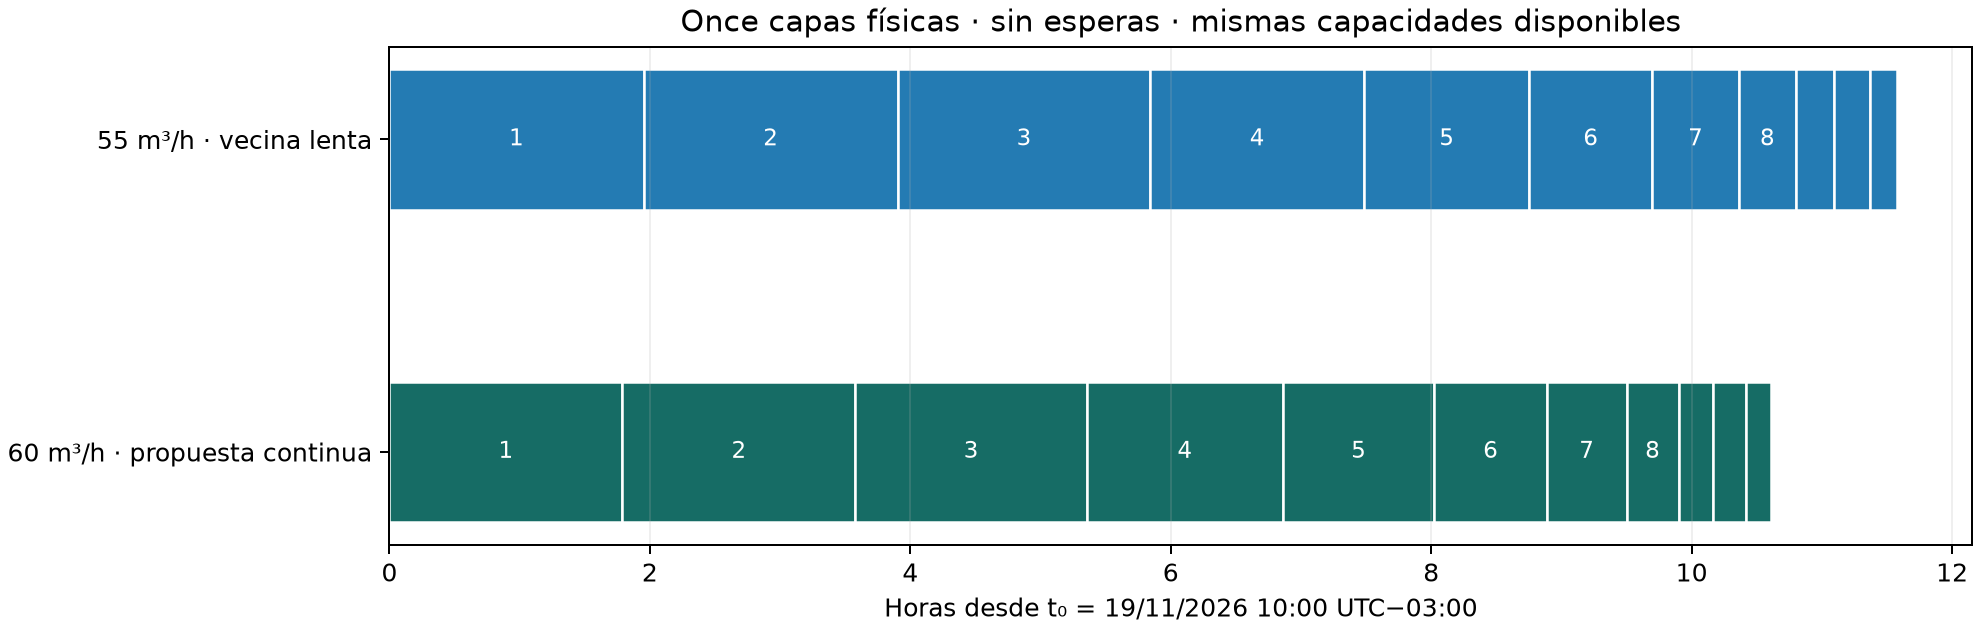
\includegraphics[width=0.98\linewidth]{Imagenes/resultados_02_CRONOGRAMAS.png}
  \caption{Secuencia continua de colocación de los dos planes finales}
  \label{fig:cronogramas-resultados}
  \captionsetup{skip=2pt}
  \caption*{Fuente: elaboración propia a partir del cronograma físico de las capas.}
\end{figure}
En el Anexo~\ref{an:detalles}, las Tablas~\ref{tab:cronograma-60} y~\ref{tab:cronograma-55} permiten trasladar la programación a cada frente. Los tiempos son horas desde $t_0$. Por ejemplo, en la propuesta el retiro de la última manta empieza a las $504\,\mathrm h$ en la primera capa y llega a la última a las $514{,}421\,\mathrm h$. Cada capa pasa entonces a sombra, que permanece hasta terminar el seguimiento.


\subsection{Probabilidades y máximos de cada plan}
La Tabla~\ref{tab:resultados-planes} reúne las duraciones, las probabilidades marginales y conjunta, y los extremos de cada conjunto de $24$ escenarios. Los dos planes cumplen a las $336$ y a las $672\,\mathrm h$. Entre ellos, la propuesta reduce la duración en $57{,}89\,\mathrm{min}$ sin aumentar la proporción de escenarios que exceden.
\begin{table}[htbp]
  \centering
  \caption{Duración, probabilidades y extremos del conjunto a $672\,\mathrm h$}
  \label{tab:resultados-planes}
  \small
  \setlength{\tabcolsep}{4pt}
  \begin{tabular}{lccccccc}
    \toprule
    Plan & $D$ [h] & $P_T$ & $P_\Delta$ & $P_f$ & Cumple & Mayor $M_T$ [$^\circ$C] & Mayor $M_\Delta$ [K] \\
    \midrule
    Propuesta base & $10{,}6129$ & $0$ & $0$ & $0$ & Sí & $47{,}4941$ & $16{,}5306$ \\
    Variante lenta & $11{,}5777$ & $0$ & $0$ & $0$ & Sí & $47{,}5128$ & $16{,}6011$ \\
    Propuesta fina & $10{,}6129$ & $0$ & $0$ & $0$ & Sí & $47{,}0322$ & $15{,}7202$ \\
    \bottomrule
  \end{tabular}
  \captionsetup{skip=2pt}
  \caption*{Fuente: elaboración propia a partir de las matrices finales de simulación.}
\end{table}
En la propuesta fina, la temperatura más alta fue de $47{,}03\,^\circ\mathrm C$ a las $126\,\mathrm h$, con \texttt{M4\_SS} y el clima de $2025$. El máximo diferencial, $15{,}72\,\mathrm K$, apareció a las $260{,}917\,\mathrm h$ con la misma curva y el clima de $2023$. En ese instante, el punto caliente alcanzó $40{,}73\,^\circ\mathrm C$ y el punto frío próximo al contorno, $25{,}01\,^\circ\mathrm C$.

La Tabla~\ref{tab:localizacion-maximos} identifica ambos puntos en coordenadas locales. Para el máximo absoluto de temperatura solo interviene $\vec x_T$; para el diferencial se necesitan $\vec x_T$ y $\vec x_{25}$ al mismo instante. La cota numérica de $4{,}40\,\mathrm m$ corresponde al contorno escalonado de la malla, mientras que el IFC alcanza $4{,}30\,\mathrm m$.
\begin{table}[htbp]
  \centering
  \caption{Escenarios, tiempos y posiciones de los extremos a $672\,\mathrm h$ ($M_T$ en $^\circ\mathrm C$ y $M_\Delta$ en $\mathrm K$)}
  \label{tab:localizacion-maximos}
  \small
  \setlength{\tabcolsep}{4pt}
  \begin{tabular}{L{1.5cm}L{1.2cm}L{1.15cm}L{1.2cm}L{1.8cm}L{3.3cm}L{3.3cm}}
    \toprule
    Plan & Métrica & Valor & Tiempo [h] & Escenario & $\vec x_T$ [m] & $\vec x_{25}$ [m] \\
    \midrule
    Propuesta base & $M_T$ & $47{,}4941$ & $125{,}000$ & \texttt{M4\_SS}, ERA5-$2025$ & $(2{,}000;0{,}000;4{,}400)$ & --- \\
    Propuesta base & $M_\Delta$ & $16{,}5306$ & $267{,}000$ & \texttt{M4\_SS}, ERA5-$2024$ & $(0{,}000;0{,}000;4{,}400)$ & $(-3{,}600;-8{,}800;0{,}025)$ \\
    Variante lenta & $M_T$ & $47{,}5128$ & $125{,}000$ & \texttt{M4\_SS}, ERA5-$2025$ & $(2{,}000;0{,}000;4{,}400)$ & --- \\
    Variante lenta & $M_\Delta$ & $16{,}6011$ & $267{,}000$ & \texttt{M4\_SS}, ERA5-$2024$ & $(0{,}000;0{,}000;4{,}400)$ & $(-3{,}600;-8{,}800;0{,}025)$ \\
    Propuesta fina & $M_T$ & $47{,}0322$ & $126{,}000$ & \texttt{M4\_SS}, ERA5-$2025$ & $(2{,}300;0{,}100;4{,}400)$ & --- \\
    Propuesta fina & $M_\Delta$ & $15{,}7202$ & $260{,}917$ & \texttt{M4\_SS}, ERA5-$2023$ & $(0{,}100;0{,}100;4{,}100)$ & $(3{,}700;-8{,}900;0{,}025)$ \\
    \bottomrule
  \end{tabular}
  \captionsetup{skip=2pt}
  \caption*{Fuente: elaboración propia a partir del cronograma y los resultados archivados de simulación.}
\end{table}


\subsection{Evolución del núcleo, del contorno y del diferencial}
La Figura~\ref{fig:curvas-resultados} sigue una sola realización, \texttt{M4\_SS} con el clima de $2024$, en las dos tasas y con idéntica resolución. El panel superior muestra el punto más caliente y el más frío de $S_{25}$; el central sigue una sonda fija del núcleo en $(0;0;2)\,\mathrm m$. El inferior muestra la diferencia simultánea y su límite.
\begin{figure}[htbp]
  \centering
  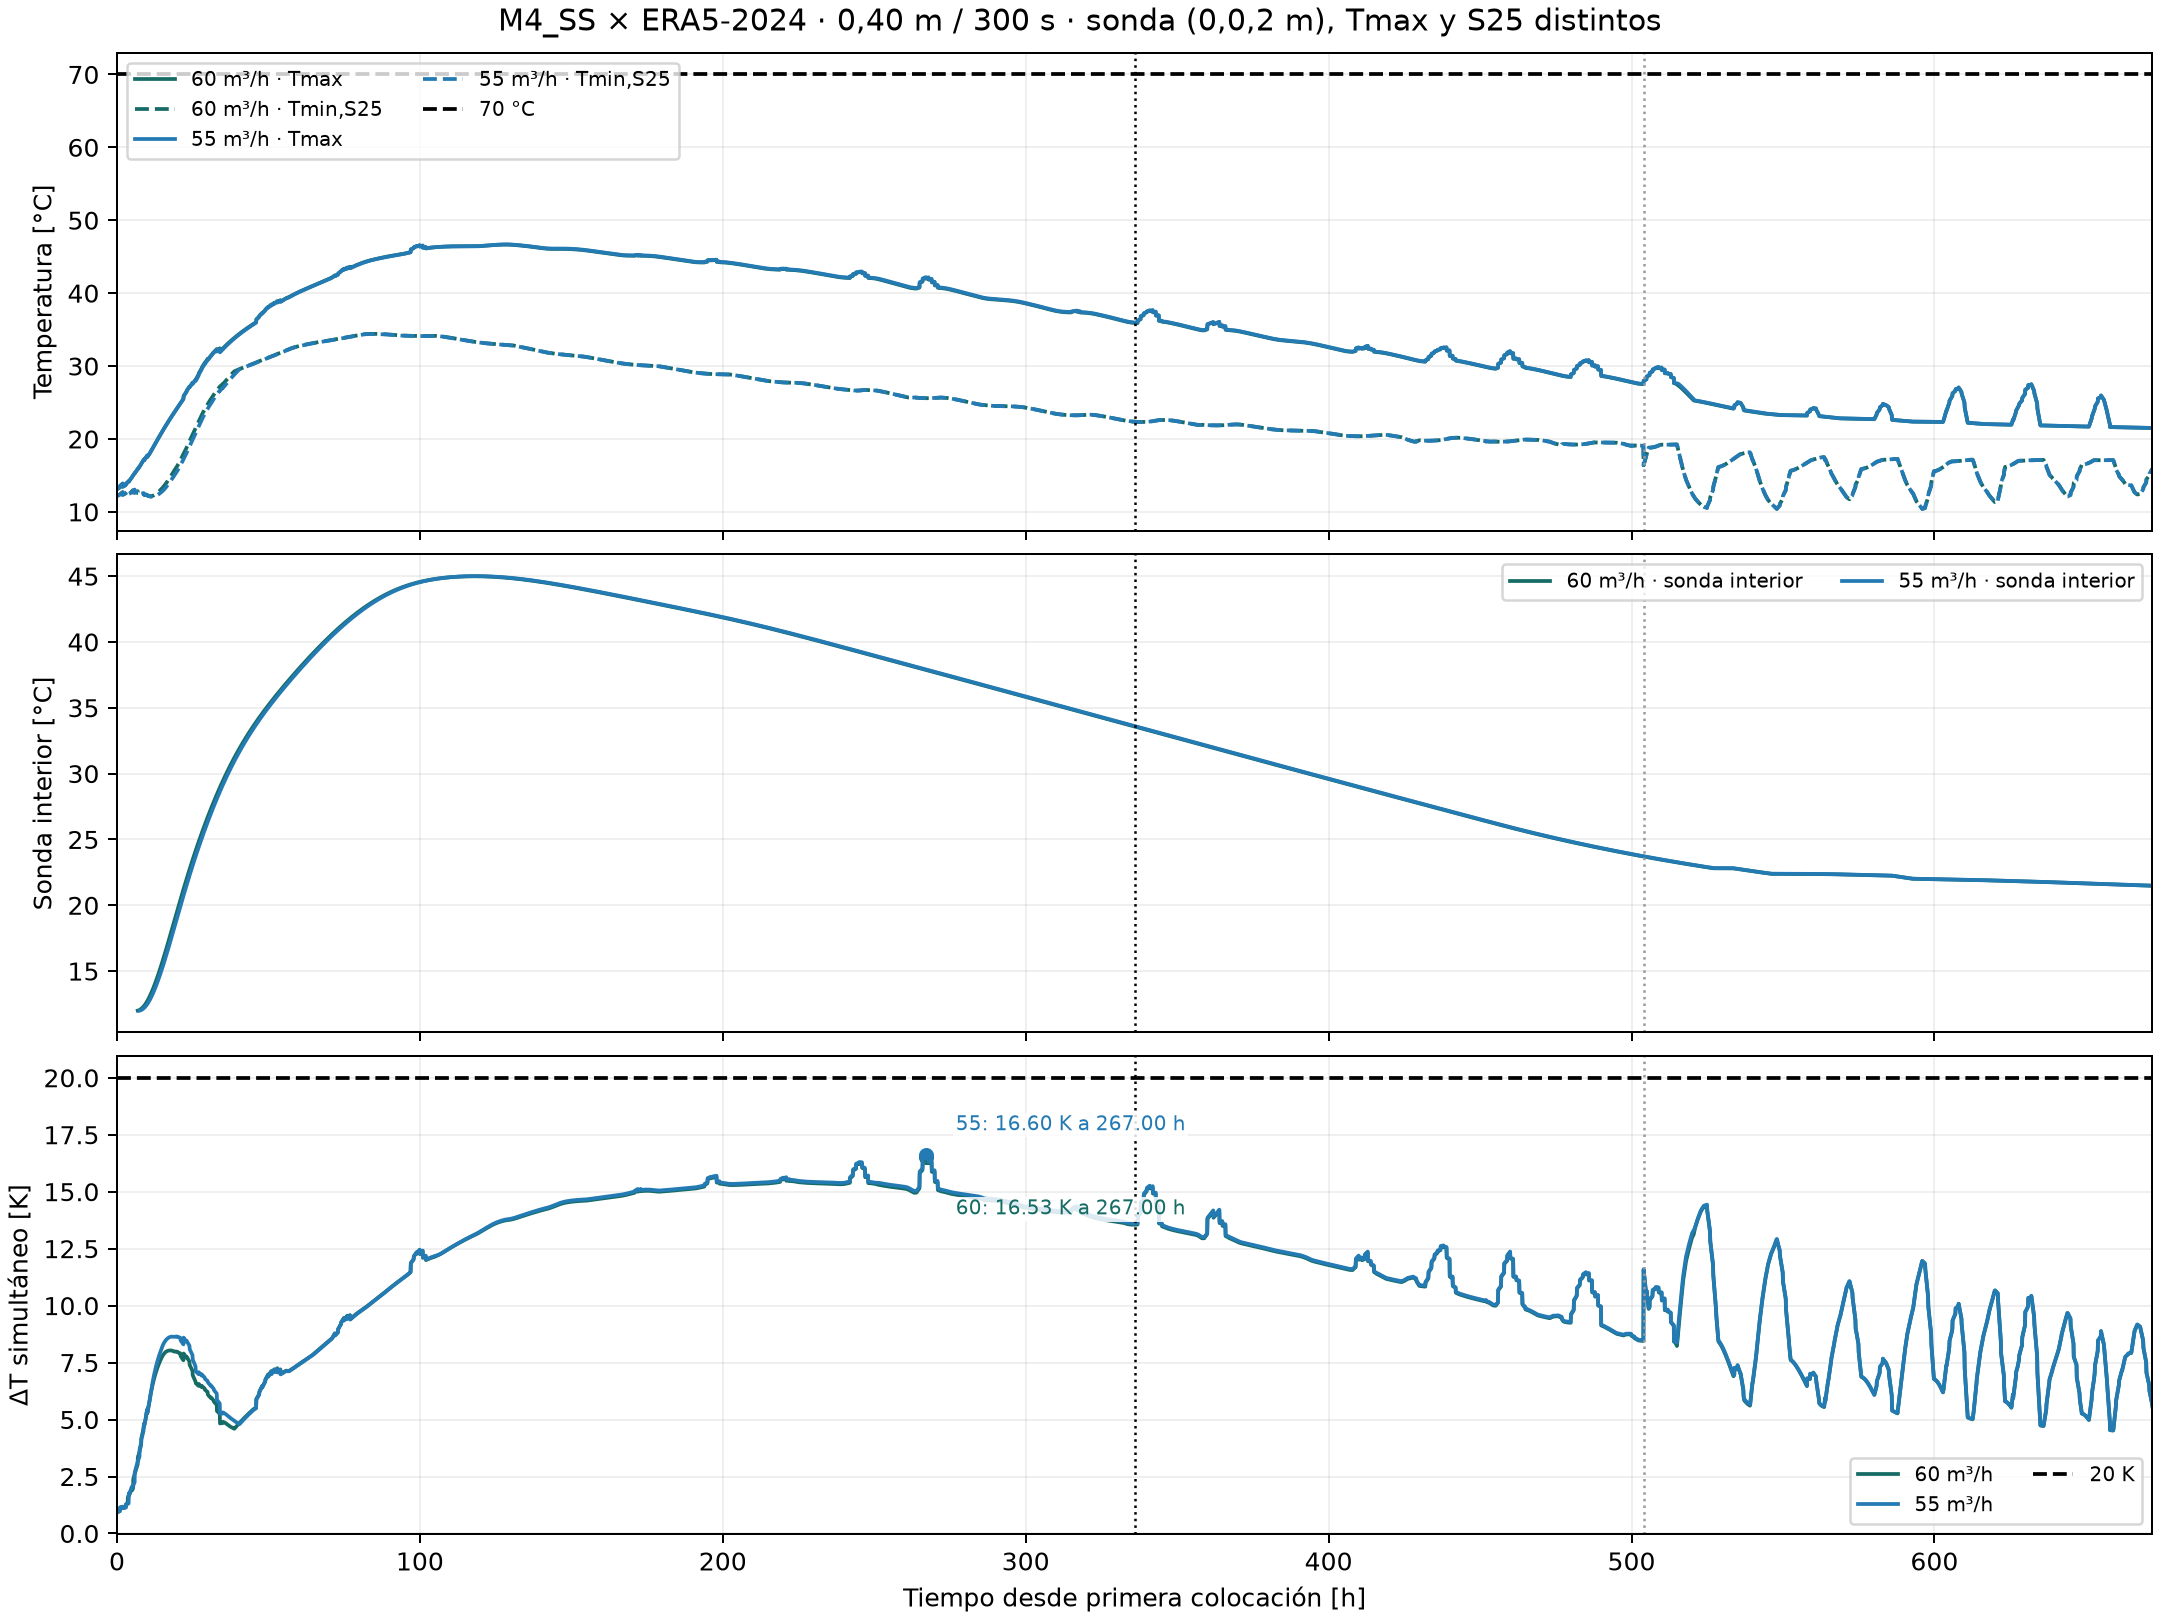
\includegraphics[width=0.98\linewidth]{Imagenes/resultados_03_CURVAS_COMPARABLES.png}
  \caption{Evolución térmica de una misma realización para los planes de $60$ y $55\,\mathrm{m^3/h}$}
  \label{fig:curvas-resultados}
  \captionsetup{skip=2pt}
  \caption*{Fuente: elaboración propia a partir de las historias térmicas de las simulaciones.}
\end{figure}
El núcleo se calienta durante las primeras edades y después se enfría más despacio que el contorno. A las $267\,\mathrm h$, el diferencial alcanza $16{,}53\,\mathrm K$ en la propuesta y $16{,}60\,\mathrm K$ en la alternativa lenta. Tras retirar la última manta crecen las oscilaciones cerca de la superficie. La línea de $504\,\mathrm h$ marca el primer retiro de esa manta.

\subsection{Campos térmicos y zonas críticas}
Los cortes de la Figura~\ref{fig:cortes-resultados} usan los mismos instantes y la misma escala de color. A las $267\,\mathrm h$ persiste una región cálida en la zona superior e interior, mientras que la base cede calor al suelo. A las $672\,\mathrm h$ el corte muestra un campo más uniforme. El punto frío que gobierna el diferencial en la malla base está cerca de $y=-8{,}80\,\mathrm m$, fuera del plano central; por eso se buscan los extremos en todo el volumen.
\begin{figure}[htbp]
  \centering
  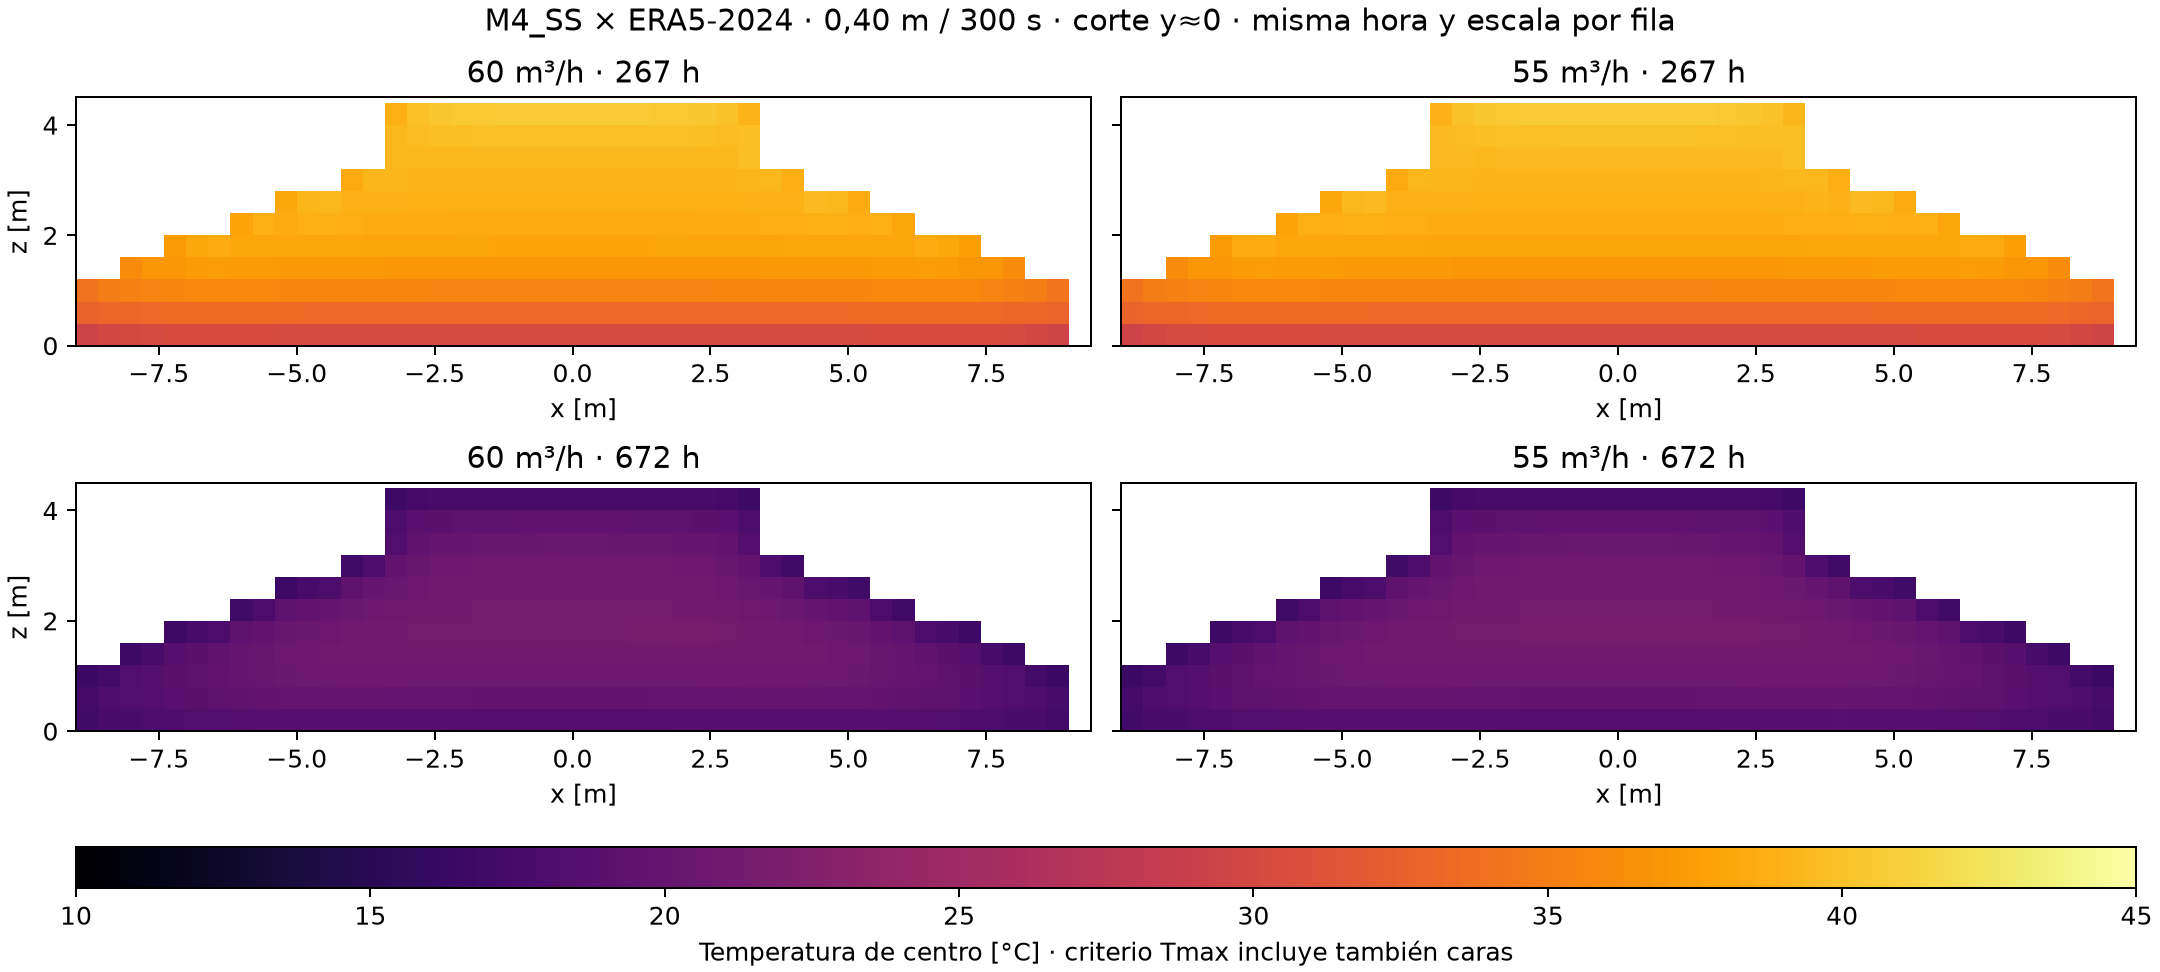
\includegraphics[width=0.98\linewidth]{Imagenes/resultados_04_CORTES_COMPARABLES_672H.png}
  \caption{Campos de temperatura en un corte central a $267$ y $672\,\mathrm h$}
  \label{fig:cortes-resultados}
  \captionsetup{skip=2pt}
  \caption*{Fuente: elaboración propia a partir de los campos de temperatura archivados.}
\end{figure}

\subsection{Relación entre duración, riesgo y desviaciones del plan}
En la Figura~\ref{fig:duracion-riesgo-resultados}, las dos tasas quedan por debajo de la línea del $5\,\text{\%}$ y la propuesta queda más a la izquierda por su menor duración. A tasa fija, el plazo es el mismo con las tres estrategias de protección, pero su resultado térmico cambia considerablemente.
\begin{figure}[htbp]
  \centering
  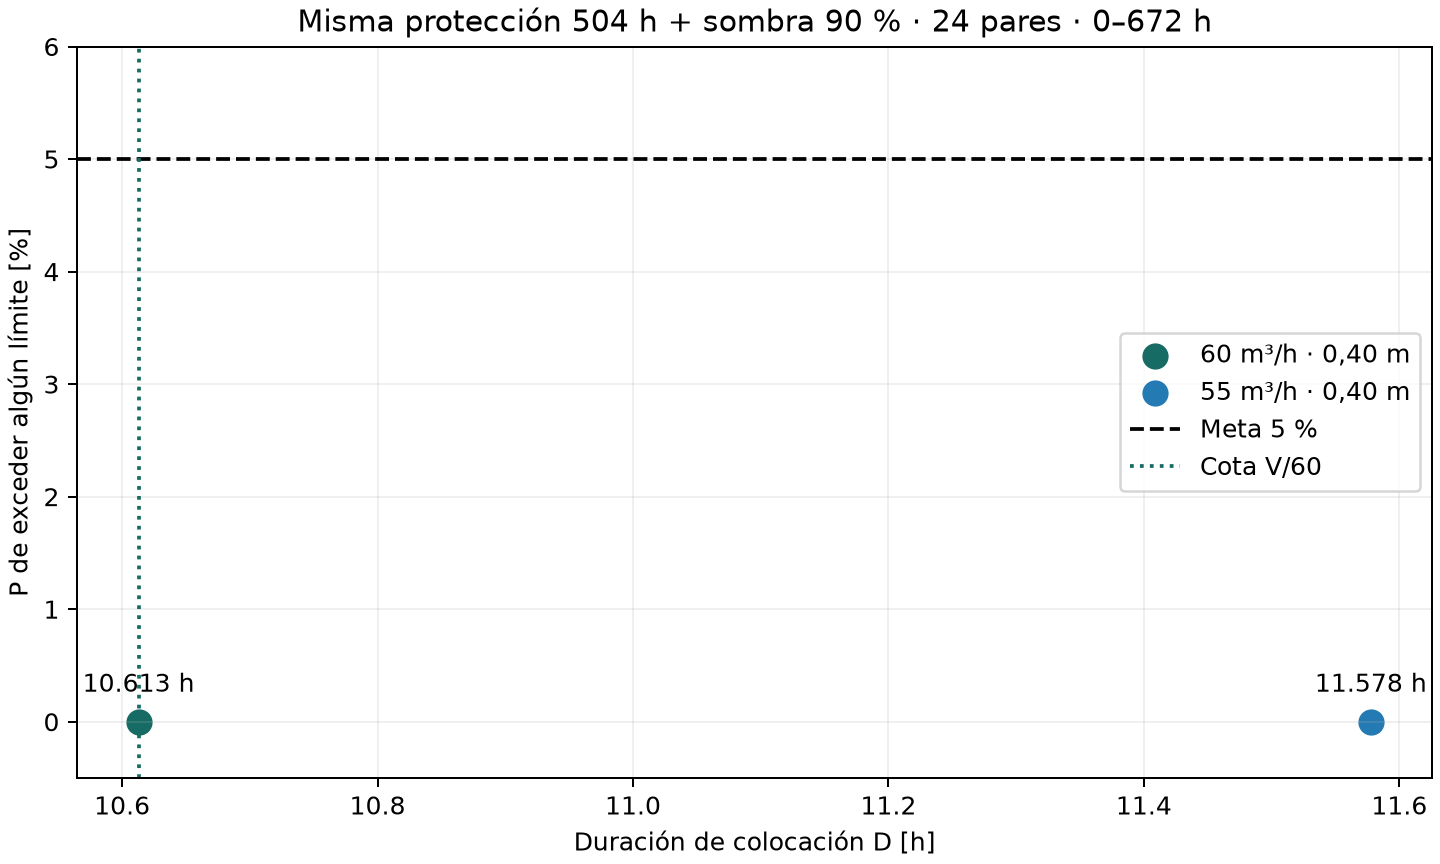
\includegraphics[width=0.90\linewidth]{Imagenes/resultados_01_D_VS_PROBABILIDAD.png}
  \caption{Duración y probabilidad conjunta de los planes finales, con la propuesta elegida en la cota $V/60$}
  \label{fig:duracion-riesgo-resultados}
  \captionsetup{skip=2pt}
  \caption*{Fuente: elaboración propia a partir de las duraciones y probabilidades de los planes.}
\end{figure}
Mantener la última manta hasta $504\,\mathrm h$ y prescindir de sombra produjo excedencias en los $24$ pares. Algunos máximos tardíos seguían pendientes, aunque la clasificación ya estaba decidida. Con sombra y retiro a $360\,\mathrm h$ excedieron $5$ de los $24$ pares ($20{,}83\,\text{\%}$). Al combinar la sombra con el retiro a $504\,\mathrm h$, ninguno excedió. Las cifras corresponden a la misma malla base, el mismo horizonte de $672\,\mathrm h$ y una duración de colocación de $10{,}6129\,\mathrm h$.

\subsection{Sensibilidades y fundamento de la elección}
La Figura~\ref{fig:sensibilidad-resultados} compara el máximo diferencial de cada escenario entre las dos mallas. El mayor cambio observado, $0{,}882\,\mathrm K$, deja la elección del mismo lado del umbral en los $24$ pares. La sensibilidad a los pesos de la Tabla~\ref{tab:sensibilidad-pesos} conserva también la decisión.
\begin{figure}[htbp]
  \centering
  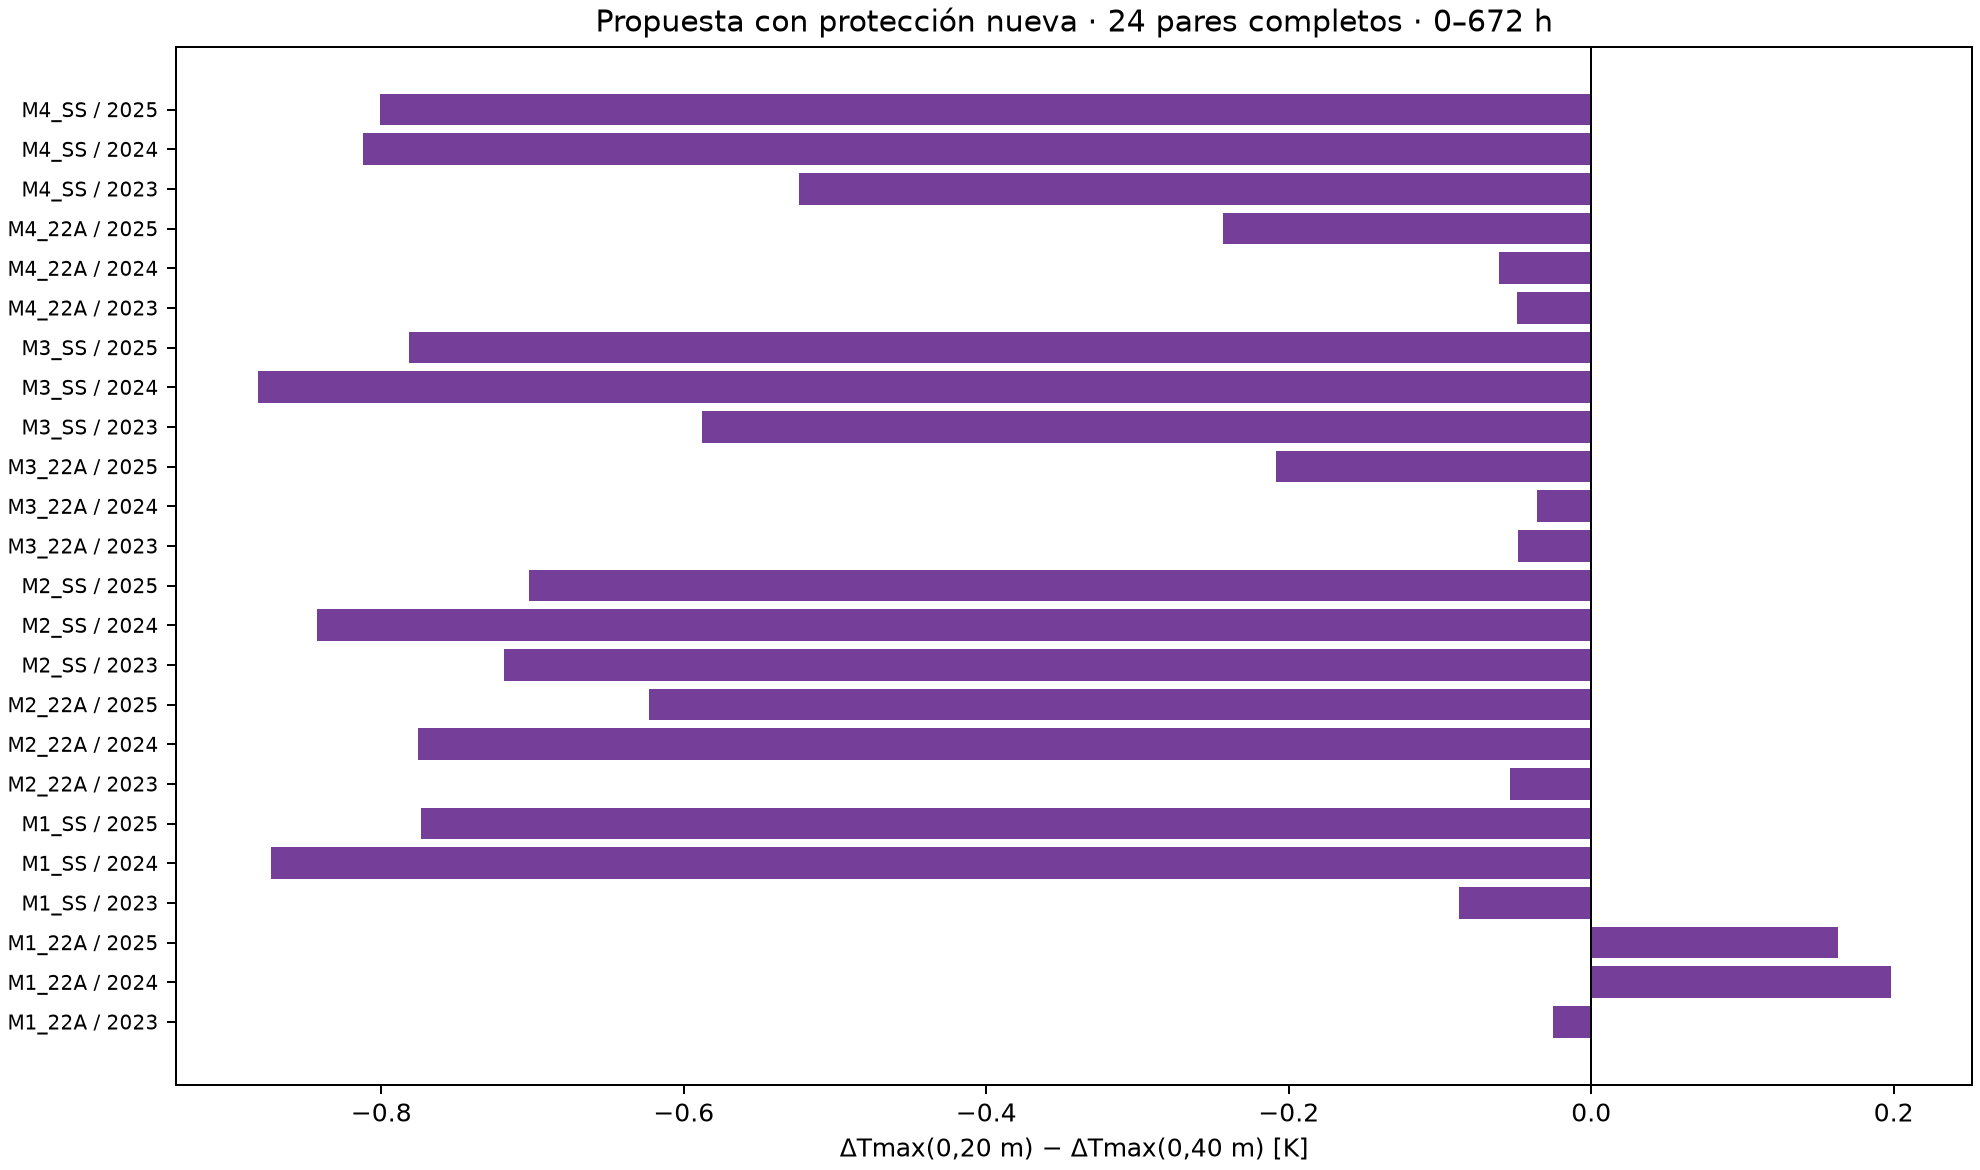
\includegraphics[width=0.95\linewidth]{Imagenes/resultados_05_SENSIBILIDAD_24_PARES.png}
  \caption{Cambio del diferencial máximo entre mallas para los $24$ escenarios de la propuesta}
  \label{fig:sensibilidad-resultados}
  \captionsetup{skip=2pt}
  \caption*{Fuente: elaboración propia a partir de las comparaciones de cada escenario en ambas mallas.}
\end{figure}
Cada barra compara máximos de una misma realización. Promediar primero los campos de temperatura suavizaría las diferencias entre años y curvas y podría ocultar precisamente una excedencia. La elección utiliza la duración física y la distribución de máximos individuales.

\section{Discusión y plan de control resultante}
\label{sec:discusion-control}

\subsection{Interpretación del comportamiento térmico}
Al principio de la colocación, el calor de hidratación se acumula en el interior más deprisa de lo que puede salir por las caras de la fundación. A medida que disminuye la generación, el intercambio con el aire y el suelo adquiere mayor importancia. Por eso el momento crítico para el diferencial puede llegar cuando la temperatura del núcleo ya está bajando.

Cada capa inicia su propia historia de hidratación sobre hormigón que ya ha empezado a calentarse. La diferencia entre las dos tasas ensayadas apenas altera las edades relativas. Una espera prolongada sí dejaría una cara expuesta durante más tiempo y cambiaría las condiciones al colocar la siguiente capa. Su efecto requeriría una nueva evaluación.

Las mantas frenan el enfriamiento superficial y retienen calor en el conjunto. Al retirarlas, la superficie vuelve a responder con mayor rapidez al viento y al enfriamiento nocturno. La sombra limita la radiación solar diurna, mientras continúa el intercambio con el cielo. Esta combinación explica por qué tan importante como la edad de retiro es el clima que encuentra la cara recién expuesta.

\subsection{Representatividad, recursos y margen de la decisión}
Los ensayos cubren ocho respuestas de probeta y tres historias meteorológicas. La asignación de pesos iguales permite comparar los planes bajo la misma información, aunque la frecuencia real de esas condiciones se desconoce. El margen calculado de $4{,}28\,\mathrm K$ supera los cambios espaciales y temporales observados. Parte de ese margen podría consumirse por variaciones de mezcla, de transferencia en los tubos o de exposición que el cálculo mantiene fijas.

La propuesta depende también de sostener dos frentes, una recepción a $12\,^\circ\mathrm C$ y una sombra con la eficacia supuesta. La probabilidad calculada corresponde a exceder temperaturas o diferenciales. Estimar la probabilidad de fisuración exigiría representar además la resistencia, las deformaciones restringidas y las tensiones del hormigón.

\subsection{Programación operativa y autorización de retiros}
Antes de colocar, el equipo de obra debería comprobar el suministro, las protecciones, la refrigeración y los sensores. Durante las once capas deberá registrar temperatura de recepción, volumen e instantes efectivos. Ante una demora o una llegada más caliente, el responsable térmico actualizará la predicción con esas condiciones antes de decidir el siguiente paso.

Las edades locales de $72$, $240$ y $504\,\mathrm h$ sirven para programar revisiones. Para autorizar cada retiro se propone comprobar resistencia suficiente, instrumentación operativa, ausencia de alarmas y diferencial observado de hasta $18\,\mathrm K$. La predicción deberá incorporar la cara descubierta, el pronóstico vigente y al menos las siguientes $48\,\mathrm h$, incluido el enfriamiento nocturno. Si persisten dudas sobre una excedencia o un pico posterior, corresponde mantener la protección y evaluar el nuevo cronograma.

\subsection{Instrumentación, registro y responsabilidades}
La Tabla~\ref{tab:instrumentacion-control} asigna funciones a la colocación, al monitoreo y a la autorización de cambios. Se proponen sondas interiores y sensores aproximadamente a $25\,\mathrm{mm}$ de las superficies reales, en base, laterales y coronación, con redundancia en los puntos críticos. Los cortes sugieren dónde concentrar la instrumentación; las posiciones definitivas deben ajustarse a armaduras, anclajes y accesos.
\begin{table}[htbp]
  \centering
  \caption{Instrumentación y funciones propuestas para el control térmico}
  \label{tab:instrumentacion-control}
  \small
  \setlength{\tabcolsep}{4pt}
  \begin{tabular}{L{2.2cm}L{7.0cm}L{5.0cm}}
    \toprule
    Conjunto & Ubicación y finalidad & Función responsable \\
    \midrule
    Hormigón interior & Núcleo de la base y pedestal; pares redundantes en zonas calientes para seguir la acumulación y el enfriamiento & Encargado de instrumentación y monitoreo \\
    Contorno & Puntos próximos a $25\,\mathrm{mm}$ de base, laterales y coronación; caras opuestas y sectores críticos & Encargado de instrumentación y monitoreo \\
    Circuitos y agua & Temperaturas a lo largo de cada circuito; caudal y temperatura de entrada y retorno, estado de válvulas y disponibilidad del sistema & Operador de refrigeración \\
    Ambiente y protección & Aire protegido de radiación, viento representativo e inspección de mantas y sombra; radiación si se dispone de medición & Encargado de monitoreo y jefe de obra \\
    Colocación & Temperatura de recepción, volúmenes, secuencia, inicio y fin por capa & Jefe de obra y responsable de suministro \\
    Revisión térmica & Contraste con predicción, diagnóstico de alarmas y autorización de cambios o retiros & Responsable técnico del plan térmico \\
    \bottomrule
  \end{tabular}
  \captionsetup{skip=2pt}
  \caption*{Fuente: elaboración propia a partir de los resultados y controles del modelo.}
\end{table}
Se propone adquirir datos cada minuto durante la colocación, los retiros y las alarmas, y archivarlos como máximo cada cinco minutos durante todo el seguimiento. Los relojes deben estar sincronizados para que el diferencial compare lecturas simultáneas. El encargado de turno revisará los registros al menos cada hora y después de cada evento. Una alarma requiere atención inmediata y una lectura discordante debe contrastarse con el sensor redundante.

\subsection{Disparadores de contingencia y acciones}
La Tabla~\ref{tab:contingencias-control} propone advertencia a $65\,^\circ\mathrm C$ o $18\,\mathrm K$ e intervención prioritaria a $68\,^\circ\mathrm C$ o $19\,\mathrm K$. El primer nivel deja $5\,\mathrm K$ hasta el límite de temperatura y $2\,\mathrm K$ hasta el de diferencial. En el segundo nivel queda solo $1\,\mathrm K$ para el diferencial, comparable con el cambio espacial observado. Esa proximidad justifica investigar la tendencia desde el primer aviso.
\begin{table}[htbp]
  \centering
  \caption{Disparadores y respuestas propuestas ante desviaciones}
  \label{tab:contingencias-control}
  \small
  \setlength{\tabcolsep}{4pt}
  \begin{tabular}{L{3.0cm}L{7.1cm}L{4.1cm}}
    \toprule
    Disparador & Respuesta propuesta & Coordinación \\
    \midrule
    Advertencia térmica o tendencia fuera de la predicción & Suspender la autorización de retiros, verificar sensores y contrastar clima, protecciones y refrigeración; actualizar la predicción & Monitoreo y responsable térmico \\
    Nivel prioritario o excedencia observada & Activar revisión técnica inmediata, mantener vigilancia continua y definir la intervención según la causa; no continuar retiros por calendario & Responsable térmico y jefe de obra \\
    Enfriamiento del contorno, viento o daño de mantas & Revisar cobertura, fijación y humedad; evaluar restitución de protección y el diferencial que induciría cada cambio & Jefe de obra y responsable térmico \\
    Falla de caudal, válvula, agua o sensado de circuito & Comprobar el ramal y la redundancia, registrar la indisponibilidad y aplicar el procedimiento de falla definido para el equipo; reevaluar capacidad disponible & Operador de refrigeración y responsable térmico \\
    Cambio de suministro, temperatura o secuencia & Registrar las condiciones reales por capa, revisar continuidad constructiva y recalcular cronograma y respuesta térmica antes de aceptar el cambio & Jefe de obra y responsable térmico \\
    Clima fuera del conjunto representado & Incorporar la información observada y prevista como nuevos datos de evaluación, conservando la trazabilidad del catálogo original & Monitoreo y responsable térmico \\
    \bottomrule
  \end{tabular}
  \captionsetup{skip=2pt}
  \caption*{Fuente: elaboración propia como propuesta operativa derivada del análisis térmico.}
\end{table}
Un aumento de refrigeración puede bajar la máxima y, al mismo tiempo, enfriar demasiado otra zona. De forma similar, descubrir una superficie puede ampliar el diferencial. Antes de cambiar potencia, agua, sombra o aislamiento se deberá comprobar la medición y evaluar la medida con una predicción actualizada. Estas intervenciones son propuestas de contingencia.

\subsection{Condiciones que obligarían a revisar la recomendación}
La vigilancia abarca al menos las $672\,\mathrm h$ estudiadas, con seguimiento reforzado durante las $24\,\mathrm h$ posteriores a cada retiro. Para liberar definitivamente los sistemas se propone exigir resistencia suficiente, sensores válidos, al menos $24\,\mathrm h$ sin demanda de reapertura y una evaluación de la retirada durante las siguientes $48\,\mathrm h$ y hasta descartar picos relevantes. La sombra permaneció en todas las simulaciones finales, por lo que su desmontaje requiere un cálculo adicional.

Si el suministro, la refrigeración o la sombra disponibles difieren del diseño, procede estudiar cambios de preenfriamiento, capacidad, secuencia o protecciones. La recomendación solo podrá trasladarse a obra una vez comprobadas esas prestaciones y contrastada la predicción con mediciones independientes.

\clearpage
\section{Conclusiones}
\label{sec:conclusiones}

Para la fundación estudiada, la colocación continua a $60\,\mathrm{m^3/h}$ terminó en $10{,}61\,\mathrm h$ y cumplió los criterios térmicos en los $24$ escenarios. Frente al plan de $55\,\mathrm{m^3/h}$ ahorró $57{,}89\,\mathrm{min}$, equivalentes al $8{,}33\,\text{\%}$ de la duración de la alternativa más lenta. Al sostener dos frentes de $30\,\mathrm{m^3/h}$ sin esperas, la propuesta alcanzó la menor duración compatible con el volumen y la capacidad disponible.

La probabilidad conjunta calculada fue $0\,\text{\%}$ tanto a los $14$ como a los $28$ días. En la malla fina, la mayor temperatura fue $47{,}03\,^\circ\mathrm C$ y el mayor diferencial fue $15{,}72\,\mathrm K$, con un margen de $4{,}28\,\mathrm K$ respecto del criterio más cercano. Estos resultados respaldan la hipótesis de trabajo para el catálogo estudiado y la programación que mantiene la última manta hasta los $21$ días de edad local y la sombra durante el seguimiento.

La principal condición para trasladar esta decisión a obra es comprobar que se mantengan las prestaciones simuladas, especialmente el ingreso del hormigón a $12\,^\circ\mathrm C$, la extracción de los nueve circuitos y la atenuación solar de la cubierta. Las mediciones de núcleo, contorno y ambiente permitirían contrastar la predicción y fundamentar el retiro de cada protección. Quedan pendientes la validación térmica de la fundación y la evaluación de la retirada definitiva de la sombra y la refrigeración.


\clearpage
\renewcommand{\refname}{Referencias}
\renewcommand{\bibsection}{\section{\refname}}
\bibliographystyle{dcu}
\renewcommand{\harvardand}{y}
\renewcommand{\harvardurl}{URL:}
{\raggedright\linespread{1.05}\selectfont\setlength{\bibsep}{0.45em}\bibliography{Ref}}

\clearpage
\section{Anexos}
\linespread{1.15}\selectfont
\setlength{\parskip}{0.35em}
\subsection{Reproducción de la comparación}
\label{an:reproduccion}

El repositorio del proyecto se encuentra en \url{https://github.com/benjagarciag/Proyecto-2-MCOC}. La entrega de defensa está identificada en Git como \texttt{Entrega F02}.

\noindent SHA de la defensa\quad\texttt{d0ed4cd1e80a3c8ca1acf26fba0be232f3ed88d3}.

 Esta revisión del artículo reorganiza la exposición, incorpora bibliografía y facilita la consulta de la evidencia. Conserva la configuración, los resultados numéricos y la recomendación de esa entrega. El identificador de la entrega F01 se proporciona junto con el PDF al cerrar la versión en el repositorio.

\subsubsection{Lectura de la evidencia archivada}

Desde la raíz del repositorio, la carpeta \path{entregas/F02/cierre_revision_final/} reúne la documentación necesaria para consultar los resultados sin simular:
\begin{itemize}
\item \path{CONFIGURACION_FINAL_REVISADA.json} y \path{PARAMETROS_FINAL.csv} identifican la geometría, los planes, las propiedades, los controles y sus fuentes.
\item \path{COMPARACION_PLANES.csv} resume las tres matrices. \path{METRICAS_144_FILAS.csv} presenta los máximos de cada escenario, sus instantes y posiciones a $336$ y $672\,\mathrm h$. Cada combinación de curva y año pesa $1/24$ en la comparación principal.
\item \path{BALANCES_144_FILAS.csv} y \path{SENSIBILIDAD_ESPACIAL_24_PARES.csv} permiten revisar la conservación de energía y los cambios entre mallas. Las figuras numeradas de la carpeta y \path{MANIFIESTO_EVIDENCIA.json} vinculan estos resultados con sus archivos.
\end{itemize}
La carpeta \path{datos/hidratacion/} contiene las fuentes docentes. Las series históricas iniciales y complementarias se conservan en \path{datos/clima/reanalisis/} y \path{datos/clima/radiacion/}. Las tablas, las series graficadas y los metadatos del artículo se encuentran en \path{entregas/F01/articulo/datos/}. La enumeración es determinista.

\subsubsection{Entorno y comandos}

El entorno local utiliza Python $3.12.10$ en Windows. Las versiones de NumPy, IfcOpenShell y las demás dependencias figuran en \path{requirements.txt}. Desde la raíz de una copia del repositorio con historial Git, estas instrucciones de PowerShell preparan el entorno y muestran las matrices archivadas:
\begin{verbatim}
py -3.12 -m venv .venv
.\.venv\Scripts\python.exe -m pip install -r requirements.txt
$py = ".\.venv\Scripts\python.exe"
$cierre = "casos/sensibilidad_h/ejecutar_cierre_f02.py"
& $py -X utf8 -B $cierre
\end{verbatim}

La primera orden siguiente reproduce o recupera un caso de la propuesta fina. La segunda recorre las dos matrices base y la matriz fina. Los resultados compatibles se reutilizan. La tercera ejecuta la auditoría de la campaña local cuando están disponibles sus archivos de ejecución.
\begin{verbatim}
& $py -X utf8 -B $cierre --ejecutar --escenario M4_SS ERA5-2024
& $py -X utf8 -B $cierre --comparar --ejecutar
& $py -X utf8 -B $cierre --auditar
\end{verbatim}

\subsection{Cronogramas por capa y detalle del cálculo}
\label{an:detalles}

\subsubsection{Secuencia de colocación y retiros}
La Figura~\ref{fig:cronogramas-resultados} compara las duraciones globales. Las Tablas~\ref{tab:cronograma-60} y~\ref{tab:cronograma-55} desglosan las once capas de cada plan, con tiempos referidos a las $10{:}00$ del $19$ de noviembre. Para trasladar un retiro al calendario se suma la edad de la protección al inicio de su capa.

\begin{table}[H]
  \centering
  \caption{Cronograma por capa del plan de $60\,\mathrm{m^3/h}$}
  \label{tab:cronograma-60}
  \small
  \setlength{\tabcolsep}{4pt}
  \begin{tabular}{ccccccc}
    \toprule
    Capa & Inicio [h] & Fin [h] & Duración [h] & Madera [h] & Manta 1 [h] & Manta 2 [h] \\
    \midrule
    $1$ & $0{,}000$ & $1{,}789$ & $1{,}789$ & $72{,}000$ & $240{,}000$ & $504{,}000$ \\
    $2$ & $1{,}789$ & $3{,}579$ & $1{,}789$ & $73{,}789$ & $241{,}789$ & $505{,}789$ \\
    $3$ & $3{,}579$ & $5{,}356$ & $1{,}777$ & $75{,}579$ & $243{,}579$ & $507{,}579$ \\
    $4$ & $5{,}356$ & $6{,}861$ & $1{,}505$ & $77{,}356$ & $245{,}356$ & $509{,}356$ \\
    $5$ & $6{,}861$ & $8{,}024$ & $1{,}163$ & $78{,}861$ & $246{,}861$ & $510{,}861$ \\
    $6$ & $8{,}024$ & $8{,}889$ & $0{,}865$ & $80{,}024$ & $248{,}024$ & $512{,}024$ \\
    $7$ & $8{,}889$ & $9{,}500$ & $0{,}611$ & $80{,}889$ & $248{,}889$ & $512{,}889$ \\
    $8$ & $9{,}500$ & $9{,}901$ & $0{,}401$ & $81{,}500$ & $249{,}500$ & $513{,}500$ \\
    $9$ & $9{,}901$ & $10{,}165$ & $0{,}264$ & $81{,}901$ & $249{,}901$ & $513{,}901$ \\
    $10$ & $10{,}165$ & $10{,}421$ & $0{,}256$ & $82{,}165$ & $250{,}165$ & $514{,}165$ \\
    $11$ & $10{,}421$ & $10{,}613$ & $0{,}192$ & $82{,}421$ & $250{,}421$ & $514{,}421$ \\
    \bottomrule
  \end{tabular}
  \captionsetup{skip=2pt}
  \caption*{Fuente: elaboración propia a partir del cronograma y los resultados archivados de simulación.}
\end{table}

\begin{table}[H]
  \centering
  \caption{Cronograma por capa del plan de $55\,\mathrm{m^3/h}$}
  \label{tab:cronograma-55}
  \small
  \setlength{\tabcolsep}{4pt}
  \begin{tabular}{ccccccc}
    \toprule
    Capa & Inicio [h] & Fin [h] & Duración [h] & Madera [h] & Manta 1 [h] & Manta 2 [h] \\
    \midrule
    $1$ & $0{,}000$ & $1{,}952$ & $1{,}952$ & $72{,}000$ & $240{,}000$ & $504{,}000$ \\
    $2$ & $1{,}952$ & $3{,}904$ & $1{,}952$ & $73{,}952$ & $241{,}952$ & $505{,}952$ \\
    $3$ & $3{,}904$ & $5{,}843$ & $1{,}939$ & $75{,}904$ & $243{,}904$ & $507{,}904$ \\
    $4$ & $5{,}843$ & $7{,}485$ & $1{,}642$ & $77{,}843$ & $245{,}843$ & $509{,}843$ \\
    $5$ & $7{,}485$ & $8{,}754$ & $1{,}269$ & $79{,}485$ & $247{,}485$ & $511{,}485$ \\
    $6$ & $8{,}754$ & $9{,}697$ & $0{,}943$ & $80{,}754$ & $248{,}754$ & $512{,}754$ \\
    $7$ & $9{,}697$ & $10{,}363$ & $0{,}666$ & $81{,}697$ & $249{,}697$ & $513{,}697$ \\
    $8$ & $10{,}363$ & $10{,}801$ & $0{,}437$ & $82{,}363$ & $250{,}363$ & $514{,}363$ \\
    $9$ & $10{,}801$ & $11{,}089$ & $0{,}289$ & $82{,}801$ & $250{,}801$ & $514{,}801$ \\
    $10$ & $11{,}089$ & $11{,}368$ & $0{,}279$ & $83{,}089$ & $251{,}089$ & $515{,}089$ \\
    $11$ & $11{,}368$ & $11{,}578$ & $0{,}209$ & $83{,}368$ & $251{,}368$ & $515{,}368$ \\
    \bottomrule
  \end{tabular}
  \captionsetup{skip=2pt}
  \caption*{Fuente: elaboración propia a partir del cronograma y los resultados archivados de simulación.}
\end{table}


\subsubsection{Reconstrucción de las fuentes de hidratación}
Para cada curva $m$, de potencia volumétrica $\dot q_{m,r}$ a la edad $a_r$ en segundos, el calor acumulado por unidad de volumen en la muestra $j$ es
\begin{equation}
 H_{m,j}=\sum_{r=0}^{j-1}\frac{\dot q_{m,r}+\dot q_{m,r+1}}{2}(a_{r+1}-a_r).
\end{equation}
Se interpola linealmente este acumulado. La pendiente del segmento es la fuente efectiva, constante dentro del intervalo correspondiente. La diferencia entre los acumulados de dos edades da la energía generada por unidad de volumen durante un paso, incluso si este atraviesa más de un intervalo de muestreo.

\subsubsection{Balance de la cara exterior y estabilidad}
Si $\mathcal F$ denota el flujo ambiental de la ecuación~\eqref{eq:balance-exterior}, la temperatura superficial se obtiene anulando
\begin{equation}
 F_f(T_s)=\frac{T_s-T_i^n}{R_{i,f}}-\mathcal F(T_s).
\end{equation}
En cada iteración se divide el residuo por la derivada $R_{i,f}^{-1}+h_c+4\varepsilon\sigma T_{s,K}^3$ y se resta la corrección a la temperatura anterior. La sensibilidad del flujo entrante de la cara a la temperatura de la celda queda acotada por
\begin{equation}
 \left|\frac{\partial(A_f\phi_f)}{\partial T_i}\right|
 =\frac{A_f(h_c+4\varepsilon\sigma T_{s,K}^3)}
 {1+R_{i,f}(h_c+4\varepsilon\sigma T_{s,K}^3)}
 \leq\frac{A_f}{R_{i,f}}.
\end{equation}
La suma de conductancias que determina el paso de la ecuación~\eqref{eq:paso-utilizado} es
\begin{equation}
 S_i=\sum_{j\in\mathcal N_i}G_{ij}
 +\sum_{f\in\mathcal B_{i,a}}A_f/R_{i,f}
 +\sum_{f\in\mathcal B_{i,g}}G_{g,f}+\chi_{r,i}U_vV_i.
\end{equation}
Los conjuntos $\mathcal B_{i,a}$ y $\mathcal B_{i,g}$ contienen las caras al aire y al suelo, respectivamente. La función $\chi_{r,i}$ distingue las celdas refrigerables. El último término se incluye aunque el circuito esté cerrado, de modo que abrirlo conserve el margen de estabilidad previsto.

\subsubsection{Temperatura efectiva del cielo}
La temperatura radiativa del cielo se estima a partir del punto de rocío $T_{d,K}$ en kelvin y la nubosidad $N$ en décimas \citep{energyplusCielo}. Se utiliza la nubosidad total como aproximación de la opaca:
\begin{equation}\begin{aligned}
  \varepsilon_{\mathrm{sky}}^*&=
  \left[0{,}787+0{,}764\ln\left(\frac{T_{d,K}}{273\,\mathrm K}\right)\right]
  \left(1+0{,}0224N-0{,}0035N^2+0{,}00028N^3\right),\\
  \varepsilon_{\mathrm{sky}}&=\min(1,\max(0,\varepsilon_{\mathrm{sky}}^*)),
  \qquad T_{\mathrm{sky},K}^4=\varepsilon_{\mathrm{sky}}T_{a,K}^4.
\end{aligned}\end{equation}


\end{document}
